% ============================================================================
% COMPETITION RIFLE BALLISTICS: A COMPREHENSIVE MANUAL
% Version 2.0 - With Reloading Implications Chapter
% ============================================================================
\documentclass[11pt,twoside,openright]{report}

% --- Geometry & Layout ---
\usepackage[a4paper,margin=2.5cm,inner=3cm,outer=2.5cm,headheight=14pt]{geometry}
\usepackage{fancyhdr}
\usepackage{titlesec}
\usepackage{tocloft}
\usepackage{parskip}

% --- Mathematics ---
\usepackage{amsmath,amssymb,amsfonts,mathtools}
\mathtoolsset{showonlyrefs}
\usepackage{bm}
\usepackage{cancel}

% --- Tables ---
\usepackage{booktabs,longtable,multirow,array,tabularx}

% --- Graphics ---
\usepackage{graphicx,xcolor,float,caption,subcaption}
\usepackage{tikz,pgfplots}
\pgfplotsset{compat=1.18}
\usetikzlibrary{arrows.meta,calc,patterns,positioning,decorations.markings}

% --- Units ---
\usepackage{siunitx}
\sisetup{per-mode=fraction,inter-unit-product=\ensuremath{\cdot}}
\DeclareSIUnit\grain{gr}
\DeclareSIUnit\inch{in}
\DeclareSIUnit\foot{ft}
\DeclareSIUnit\yard{yd}
\DeclareSIUnit\moa{MOA}
\DeclareSIUnit\mil{mil}
\DeclareSIUnit\fps{ft/s}
\DeclareSIUnit\mph{mph}
\DeclareSIUnit\lbf{lbf}
\DeclareSIUnit\psi{psi}

% --- Code listings ---
\usepackage{listings}
\definecolor{jlpurple}{RGB}{149,88,178}
\definecolor{jlgreen}{RGB}{56,132,78}
\definecolor{jlblue}{RGB}{48,99,176}
\definecolor{jlgray}{RGB}{240,240,240}
\lstdefinelanguage{Julia}{
  keywords={function,end,if,else,elseif,for,while,return,struct,mutable,const,
            module,export,using,import,begin,let,do,try,catch,finally,true,false,nothing},
  keywordstyle=\color{jlpurple}\bfseries,
  ndkeywords={Float64,Int64,Vector,Dict,Tuple,String,Bool,Any,Real,AbstractFloat,
              println,sqrt,exp,log,sin,cos,tan,asin,acos,atan,abs,sign,
              push!,zeros,ones,range,collect,map,sum,maximum,minimum},
  ndkeywordstyle=\color{jlblue}\bfseries,
  sensitive=true,
  comment=[l]{\#},
  commentstyle=\color{jlgreen}\itshape,
  stringstyle=\color{red!70!black},
  string=[b]",
  morestring=[b]',
}
\lstset{
  language=Julia,
  basicstyle=\small\ttfamily,
  backgroundcolor=\color{jlgray},
  frame=single,
  rulecolor=\color{gray!50},
  numbers=left,
  numberstyle=\tiny\color{gray},
  numbersep=8pt,
  breaklines=true,
  breakatwhitespace=false,
  tabsize=4,
  showstringspaces=false,
  captionpos=b,
  aboveskip=10pt,
  belowskip=10pt,
}

% --- Hyperlinks ---
\usepackage[colorlinks=true,linkcolor=blue!60!black,citecolor=green!40!black,
            urlcolor=blue!70!black,bookmarks=true,bookmarksnumbered=true]{hyperref}

% --- Bibliography ---
\usepackage{natbib}
\bibliographystyle{plainnat}

% --- Enumeration ---
\usepackage{enumitem}

% --- Header/Footer ---
\pagestyle{fancy}
\fancyhf{}
\fancyhead[LE]{\leftmark}
\fancyhead[RO]{\rightmark}
\fancyfoot[C]{\thepage}
\renewcommand{\headrulewidth}{0.4pt}

% --- Chapter formatting ---
\titleformat{\chapter}[display]
  {\normalfont\huge\bfseries}{\chaptertitlename\ \thechapter}{20pt}{\Huge}
\titlespacing*{\chapter}{0pt}{-20pt}{40pt}

% --- Custom commands ---
\newcommand{\dd}{\mathrm{d}}
\newcommand{\Cd}{C_{\mathrm{D}}}
\newcommand{\Bc}{B_{\mathrm{C}}}
\newcommand{\vvec}{\bm{v}}
\newcommand{\avec}{\bm{a}}
\newcommand{\gvec}{\bm{g}}
\newcommand{\rvec}{\bm{r}}
\newcommand{\hatr}{\hat{\bm{r}}}
\newcommand{\Mach}{\mathit{Ma}}
\newcommand{\Rey}{\mathit{Re}}
\newcommand{\sd}{\mathrm{SD}}
\newcommand{\ff}{\mathrm{FF}}
\newcommand{\degF}{\ensuremath{{}^{\circ}\mathrm{F}}}
\newcommand{\degC}{\ensuremath{{}^{\circ}\mathrm{C}}}
\newcommand{\default}[1]{\;\textrm{\textcolor{blue!60!black}{[default: #1]}}}
\newcommand{\inmark}{\,\textrm{in.}}

% ============================================================================
\begin{document}

% --- Title Page ---
\begin{titlepage}
\centering
\vspace*{2cm}
{\Huge\bfseries Consolidated Competition Ballistics\\[0.5cm]
\Large A Comprehensive Mathematical Manual\\[0.3cm]
with Reloading Guide and Julia Implementations}\\[2cm]
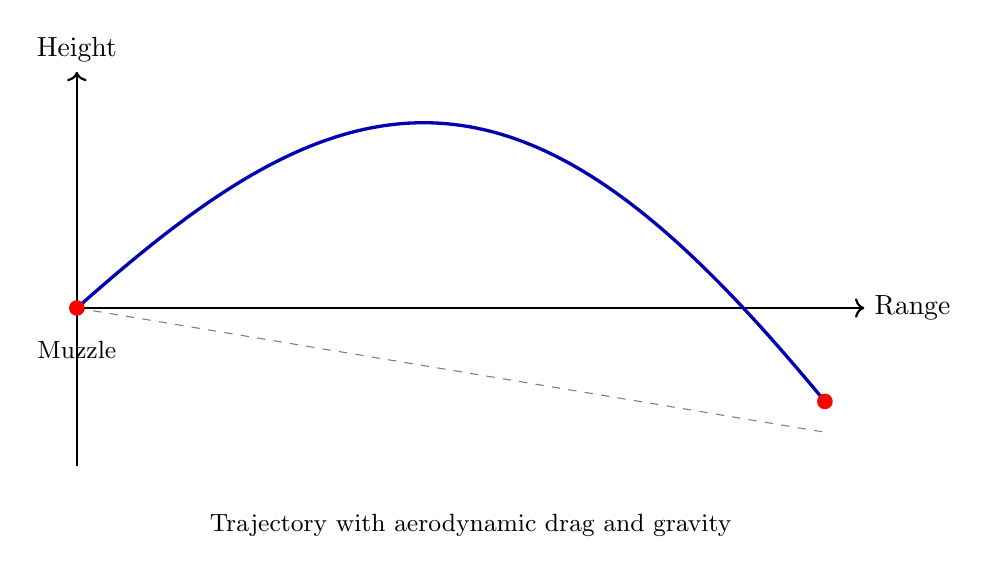
\begin{tikzpicture}
  \draw[thick,->] (0,0) -- (10,0) node[right]{Range};
  \draw[thick,->] (0,-2) -- (0,3) node[above]{Height};
  \draw[very thick, blue!70!black, domain=0:9.5, samples=100]
    plot (\x, {2.5*sin(18*\x) - 0.028*\x*\x + 0.1*\x});
  \draw[dashed, gray] (0,0) -- (9.5, {-0.028*9.5*9.5 + 0.1*9.5});
  \node[circle,fill=red,inner sep=2pt] at (0,0) {};
  \node[below] at (0,-0.3) {\small Muzzle};
  \node[circle,fill=red,inner sep=2pt] at (9.5,{2.5*sin(18*9.5) - 0.028*9.5*9.5 + 0.1*9.5}) {};
  \node[below] at (5,-2.5) {\small Trajectory with aerodynamic drag and gravity};
\end{tikzpicture}
\\[2cm]
{\large\itshape Merging Core Theory, Advanced Effects, and Practical Shooting Tools\\
Drag Models (G1--G8), Coriolis \& E\"otv\"os Effects, Spin Drift,\\
Aerodynamic Jump, Wind Deflection, and Handloading Data}\\[1.5cm]
{\large Version 3.1 (Updated) --- \today}
\end{titlepage}

\begin{abstract}
This manual provides a rigorous mathematical treatment of competition rifle ballistics. The current version (v3.1) includes significant precision improvements to the 3-DOF engine (Coordinate System alignment and 4/$\pi$ drag scaling) and outlines the roadmap for the implementation of a 6-DOF McCoy expert mode.
\end{abstract}

\pagenumbering{roman}
\tableofcontents
\newpage
\listoftables
\listoffigures
\newpage

% ============================================================================
\chapter*{Notation and Conventions}
\addcontentsline{toc}{chapter}{Notation and Conventions}
\markboth{Notation and Conventions}{Notation and Conventions}

Throughout this manual, the following conventions are used:

\begin{longtable}{@{}lll@{}}
\toprule
\textbf{Symbol} & \textbf{Meaning} & \textbf{Typical Units} \\
\midrule
\endhead
$m$ & Projectile mass & \si{\grain} or \si{\kilogram} \\
$d$ & Projectile caliber (diameter) & \si{\inch} or \si{\meter} \\
$v$, $\vvec$ & Velocity (scalar, vector) & \si{\fps} or \si{\meter\per\second} \\
$v_0$ & Muzzle velocity & \si{\fps} or \si{\meter\per\second} \\
$\Cd$ & Drag coefficient (dimensionless) & --- \\
$\Bc$ & Ballistic coefficient & \si{\lbf\per\inch\squared} \\
$\sd$ & Sectional density $= m/d^2$ & \si{\lbf\per\inch\squared} \\
$i$ or $\ff$ & Form factor (dimensionless) & --- \\
$\rho$ & Air density & \si{\kilogram\per\meter\cubed} \\
$A$ & Cross-sectional area $= \pi d^2/4$ & \si{\meter\squared} \\
$g$ & Gravitational acceleration & \si{\meter\per\second\squared} \\
$\Mach$ & Mach number $= v/a$ & --- \\
$a$ & Local speed of sound & \si{\meter\per\second} \\
$T$ & Temperature & \si{\kelvin}, \si{\celsius}, or $\degF$ \\
$P$ & Barometric pressure & \si{\hecto\pascal} or in~Hg \\
$H$ & Relative humidity & \% \\
$\theta$ & Launch (elevation) angle & \si{\degree} or \si{\mil} \\
$\phi$ & Latitude & \si{\degree} \\
$\psi$ & Azimuth (heading) & \si{\degree} \\
$\omega_E$ & Earth's angular velocity & \SI{7.2921e-5}{\radian\per\second} \\
$S_g$ & Gyroscopic stability factor & --- \\
$\tau$ & Twist rate & in.\ per turn \\
$r$ & Range & \si{\yard} or \si{\meter} \\
$\Delta y$ & Vertical drop & \si{\inch} or \si{\meter} \\
$E_k$ & Kinetic energy & \si{\joule} or ft$\cdot$lbf \\
\bottomrule
\end{longtable}

\textbf{Default values.} Parameters shown in \default{blue brackets} indicate default values used when the specific value is unknown. These are based on ICAO standard atmosphere and common competition shooting conditions.

\textbf{Unit systems.} All derivations use SI units internally. Conversion factors to Imperial units (grains, feet per second, inches, etc.) are provided throughout.

\newpage
\pagenumbering{arabic}
\setcounter{page}{1}

% ============================================================================
\chapter{Introduction to Competition Rifle Ballistics}
\label{ch:intro}

\section{Motivation: Why Math Matters in Marksmanship}

When firing a rifle at a target 100 yards away, marksmanship is almost entirely about human mechanics: trigger control, breathing, and steady hold. However, as the range stretches to 1,000 yards and beyond, marksmanship transforms into applied physics. A perfectly executed trigger pull is mathematically guaranteed to miss if the shooter has not correctly accounted for the temperature of the air, the spin of the earth, or the aerodynamic decay of their bullet. 

This manual is written for the shooter who wants to stop guessing and start calculating.

\section{Scope and Purpose}

This manual provides a rigorous mathematical treatment of the ballistic phenomena relevant to precision rifle competition, including but not limited to: F-Class, Palma, Benchrest, PRS (Precision Rifle Series), NRL (National Rifle League), High-Power, and long-range target shooting. The goal is to equip the competitive shooter with both the theoretical foundations and the practical computational tools needed to predict bullet trajectories to the highest possible accuracy.

Competition shooting demands sub-MOA accuracy at distances often exceeding \SI{1000}{\yard}. At these ranges, small errors in modeling atmospheric drag, spin drift, Coriolis deflection, or wind become dominant factors in the miss distance. This manual addresses each of these systematically.

\section{Overview of Ballistic Phases}

The flight of a bullet from ignition to impact is conventionally divided into four phases \citep{mccoy1999modern}:

\begin{enumerate}[label=\textbf{\arabic*.}]
  \item \textbf{Interior Ballistics} --- The physics of the bullet inside the barrel, from primer ignition through propellant combustion to muzzle exit. Key outputs: muzzle velocity, chamber pressure, barrel time.
  \item \textbf{Transitional (Intermediate) Ballistics} --- The brief phase as the bullet exits the muzzle and the propellant gases dissipate. Muzzle blast interaction, base drag changes, and initial yaw (tip-off) are determined here.
  \item \textbf{Exterior Ballistics} --- The free-flight trajectory from muzzle to target. This is the dominant focus of competition ballistics: aerodynamic drag, gravity drop, wind deflection, spin drift, Coriolis and E\"otv\"os effects, Magnus force, and aerodynamic jump.
  \item \textbf{Terminal Ballistics} --- Bullet behavior at impact. While less critical for paper-target competition, terminal effects matter for steel-target energy requirements and for hunting-oriented competitions.
\end{enumerate}

\section{Historical Context}

The mathematical study of projectile motion dates to Galileo and Newton, but modern exterior ballistics began with the work of Bashforth (1870), who conducted some of the earliest systematic drag measurements \citep{bashforth1870description}. The Siacci method (1880s) introduced the concept of the ballistic coefficient and drag functions that remain in use today \citep{siacci1888balistica}. In the 20th century, the US Army Ballistic Research Laboratory (BRL) at Aberdeen Proving Ground produced the definitive drag function tables---G1 through G8---that form the backbone of modern ballistic computation \citep{mccoy1999modern, ingalls1893exterior}.

Modern computational ballistics, exemplified by solvers such as those described by \citet{litz2011applied} and implemented in software like Bryan Litz's Applied Ballistics suite, use 3-DOF and 6-DOF point-mass models with empirically measured drag data and atmospheric corrections.


% ============================================================================
\chapter{Atmospheric Model}
\label{ch:atmosphere}

The atmosphere is the invisible medium through which the bullet travels. In a vacuum, a bullet would follow a perfect parabola. In reality, the air acts as a viscous fluid that constantly robs the bullet of its kinetic energy, slowing it down and exposing it to wind. Accurate modeling of air density, speed of sound, and viscosity is the absolute prerequisite to all exterior ballistic calculations.

\section{Motivation: Why Air Density is King}

A shooter might carefully measure their muzzle velocity and bullet weight, but fail to account for the environment. The primary motivation for using a precise atmospheric model is that the environment dynamically changes the aerodynamic drag fighting the bullet. 

To understand this, consider the fundamental aerodynamic drag force equation. Before we present it, let's clearly define the physical quantities involved:
\begin{itemize}[noitemsep]
    \item $F_{\text{drag}}$: The drag force opposing the bullet's motion (measured in Newtons, \si{\newton}).
    \item $\rho$ (rho): The mass density of the air the bullet is currently flying through (measured in \si{\kilogram\per\meter\cubed}).
    \item $C_d$: The drag coefficient, a dimensionless number characterizing how "slippery" the bullet is.
    \item $A$: The frontal cross-sectional area of the bullet (measured in \si{\meter\squared}).
    \item $v$: The velocity of the bullet relative to the surrounding air mass (measured in \si{\meter\per\second}).
\end{itemize}

With these defined, the drag force is expressed as:
\begin{equation}
  F_{\text{drag}} = \frac{1}{2} \rho \, C_d \, A \, v^2
  \label{eq:drag_motivation}
\end{equation}

\begin{figure}[H]
\centering
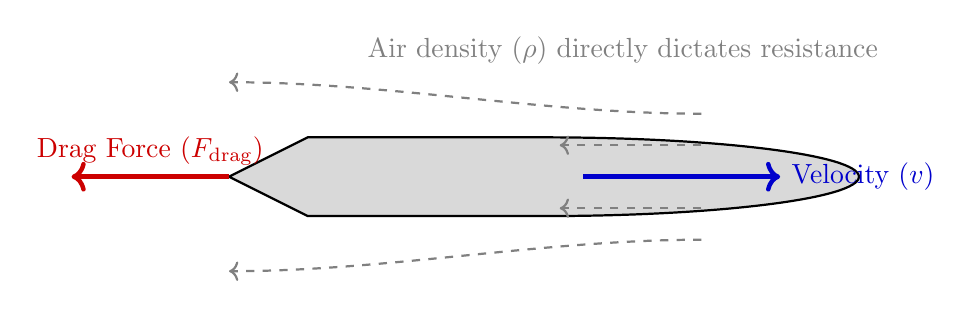
\begin{tikzpicture}
  % Bullet shape
  \draw[fill=gray!30, thick] (0,0) -- (1,0.5) -- (4,0.5) arc (90:-90:4 and 0.5) -- (1,-0.5) -- cycle;
  % Velocity vector
  \draw[->, ultra thick, blue!80!black] (4.5,0) -- (7,0) node[right] {Velocity ($v$)};
  % Drag force vector
  \draw[<-, ultra thick, red!80!black] (-2,0) -- (0,0) node[midway, above] {Drag Force ($F_{\text{drag}}$)};
  % Airflow lines
  \draw[->, gray, dashed, thick] (6, 0.8) .. controls (4, 0.8) and (2, 1.2) .. (0, 1.2);
  \draw[->, gray, dashed, thick] (6, -0.8) .. controls (4, -0.8) and (2, -1.2) .. (0, -1.2);
  \draw[->, gray, dashed, thick] (6, 0.4) -- (4.2, 0.4);
  \draw[->, gray, dashed, thick] (6, -0.4) -- (4.2, -0.4);
  \node[above, gray] at (5, 1.3) {Air density ($\rho$) directly dictates resistance};
\end{tikzpicture}
\caption{The aerodynamic drag force opposes the bullet's velocity. Notice that the force scales linearly with air density $\rho$.}
\label{fig:drag_force_diagram}
\end{figure}

As seen in Eq.~\eqref{eq:drag_motivation}, the drag force is \emph{directly proportional} to the air density $\rho$. Consequently, a 10\% error in calculating the air density results in exactly a 10\% error in the computed drag. This will directly and non-linearly affect vertical drop and wind drift.

At long ranges, these effects are substantial. For example, at 1,000 meters, the difference between typical summer (hot, thin air) and winter (cold, dense air) conditions can exceed one full meter (over 3 MOA) of vertical drop for a standard competition cartridge. By understanding and actively calculating these variables, a shooter stops relying on empirical "dope cards" and can mathematically guarantee first-round hits across varying climates.

\section{ICAO Standard Atmosphere}
\label{sec:icao}

To have a baseline for comparison, aerodynamicists and ballisticians use the International Civil Aviation Organization (ICAO) standard atmosphere. This defines standard "sea level" conditions \citep{icao1993manual,coesa1976standard}. Let's define the benchmark variables:

\begin{align}
  T_0 &= \SI{288.15}{\kelvin} \quad (\SI{15}{\celsius}, 59\,\degF) \quad \text{(Standard Temperature)} \\
  P_0 &= \SI{101325}{\pascal} \quad (29.92\;\text{in Hg}) \quad \text{(Standard Pressure)} \\
  \rho_0 &= \SI{1.2250}{\kilogram\per\meter\cubed} \quad \text{(Standard Density)} \\
  a_0 &= \SI{340.294}{\meter\per\second} \quad (\SI{1116.45}{\fps}) \quad \text{(Speed of Sound)} \\
  H_0 &= 0\% \quad \text{(Relative Humidity: completely dry air)}
\end{align}

Default values: $T_0 = 288.15\;\text{K}$ (\SI{15}{\celsius}), $P_0 = 101325\;\text{Pa}$, $\rho_0 = 1.225\;\text{kg/m}^3$, $H_0 = 0\%$.

\subsection{Temperature Lapse Rate}

Below \SI{11000}{\meter} (troposphere), the standard lapse rate is:
\begin{equation}
  T(h) = T_0 - L \cdot h, \qquad L = \SI{0.0065}{\kelvin\per\meter}
  \label{eq:lapse}
\end{equation}
where $h$ is the altitude above sea level in meters.

\subsection{Pressure--Altitude Relationship}

Using the barometric formula for the troposphere:
\begin{equation}
  P(h) = P_0 \left(\frac{T(h)}{T_0}\right)^{g_0/(L\,R_{\mathrm{air}})}
  = P_0 \left(1 - \frac{L\,h}{T_0}\right)^{5.2559}
  \label{eq:pressure_altitude}
\end{equation}
where $g_0 = \SI{9.80665}{\meter\per\second\squared}$ and $R_{\mathrm{air}} = \SI{287.0528}{\joule\per\kilogram\per\kelvin}$.

Figure~\ref{fig:isa_profile} shows how temperature, pressure, and density vary with altitude across the troposphere.

\begin{figure}[H]
\centering
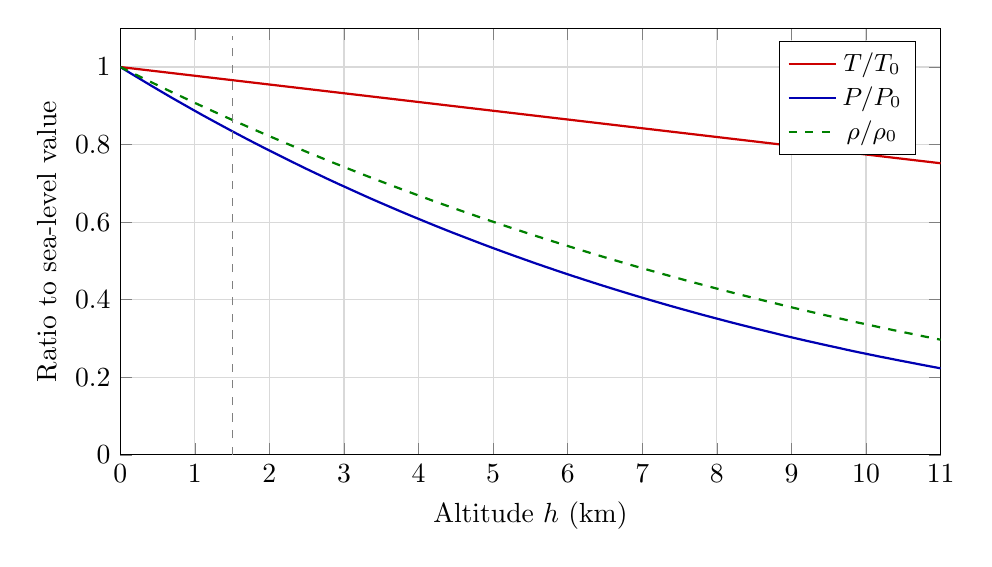
\begin{tikzpicture}
\begin{axis}[
    width=12cm, height=7cm,
    xlabel={Altitude $h$ (km)},
    ylabel={Ratio to sea-level value},
    xmin=0, xmax=11,
    ymin=0, ymax=1.1,
    grid=both,
    grid style={gray!30},
    legend pos=north east,
    legend style={font=\small},
    xtick={0,1,...,11},
]
\addplot[thick, red!80!black, domain=0:11, samples=50]
    {1 - 0.022558*x};
\addplot[thick, blue!70!black, domain=0:11, samples=80]
    {(1 - 0.022558*x)^5.2559};
\addplot[thick, green!50!black, dashed, domain=0:11, samples=80]
    {(1 - 0.022558*x)^4.2559};
\legend{$T/T_0$, $P/P_0$, $\rho/\rho_0$}
\draw[gray, thin, dashed] (axis cs:1.5,0) -- (axis cs:1.5,1.08);
\node[above, font=\scriptsize, gray] at (axis cs:1.5,1.08) {1500\,m};
\end{axis}
\end{tikzpicture}
\caption{ICAO Standard Atmosphere profiles (troposphere, 0--11\,km). Temperature decreases linearly at $L = 6.5$~K/km, while pressure and density follow power laws with exponents $n = 5.256$ and $n-1 = 4.256$ respectively. The dashed vertical line marks 1500\,m, a typical mountain shooting altitude where density is already reduced by $\approx 14$\,\%.}
\label{fig:isa_profile}
\end{figure}

\section{Air Density}

The ideal gas law gives the dry-air density:
\begin{equation}
  \rho_{\mathrm{dry}} = \frac{P}{R_{\mathrm{air}} \, T}
  \label{eq:rho_dry}
\end{equation}

\subsection{Humidity Correction}

Humid air is \emph{less dense} than dry air because water vapor ($M_{w}=\SI{18.015}{\gram\per\mole}$) is lighter than diatomic nitrogen ($M_{N_2}=\SI{28.014}{\gram\per\mole}$) and oxygen ($M_{O_2}=\SI{31.998}{\gram\per\mole}$).

The saturation vapor pressure (August--Roche--Magnus formula):
\begin{equation}
  e_s(T) = 6.1078 \times 10^{\frac{7.5\,(T - 273.15)}{T - 35.85}} \quad [\text{hPa}]
  \label{eq:sat_vapor}
\end{equation}

The partial pressure of water vapor:
\begin{equation}
  e = \frac{H}{100}\, e_s(T)
\end{equation}

Corrected density accounting for humidity (virtual temperature method):
\begin{equation}
  \rho = \frac{P - 0.3780\,e}{R_{\mathrm{air}}\,T}
  \label{eq:rho_humid}
\end{equation}
where $P$ is the total barometric pressure, $e$ is the partial pressure of water vapor, $T$ is the absolute temperature, and $R_{\mathrm{air}}$ is the specific gas constant for dry air.

The factor 0.3780 arises from $(1 - M_w/M_{\mathrm{air}}) = 1 - 18.015/28.964 \approx 0.3780$.

Figure~\ref{fig:density_sensitivity} compares the relative importance of temperature, pressure, and humidity on air density under typical field conditions.

\begin{figure}[H]
\centering
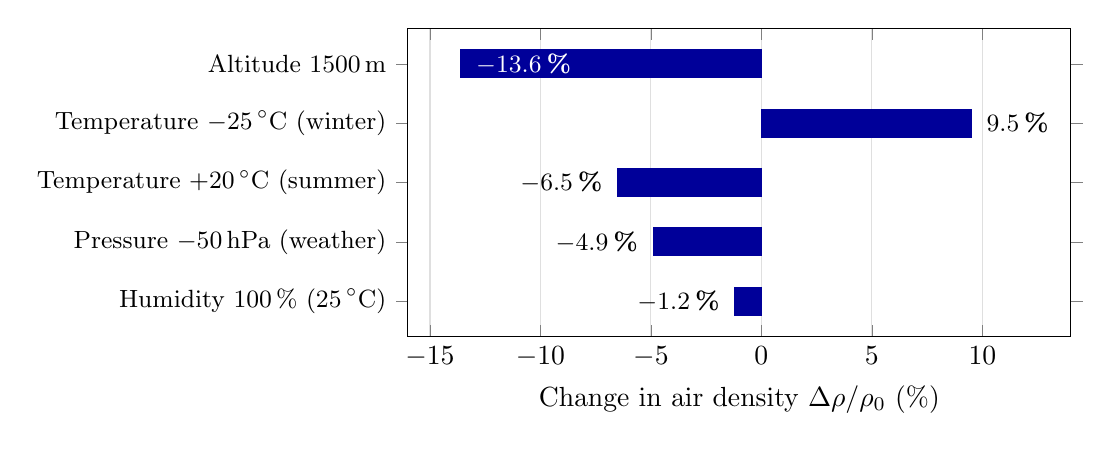
\begin{tikzpicture}
\begin{axis}[
    xbar,
    width=10cm, height=5.5cm,
    xlabel={Change in air density $\Delta\rho/\rho_0$ (\%)},
    ytick={1,2,3,4,5},
    yticklabels={
        {Humidity 100\,\% (25\,$^\circ$C)},
        {Pressure $-50$\,hPa (weather)},
        {Temperature $+20$\,$^\circ$C (summer)},
        {Temperature $-25$\,$^\circ$C (winter)},
        {Altitude 1500\,m}
    },
    y tick label style={font=\small, anchor=east},
    xmin=-16, xmax=14,
    bar width=10pt,
    xmajorgrids=true,
    ymajorgrids=false,
    grid style={gray!25},
    enlarge y limits=0.15,
]
\addplot[fill=blue!60!black, draw=blue!60!black] coordinates {
    (-1.2, 1)
    (-4.9, 2)
    (-6.5, 3)
    (9.5,  4)
    (-13.6, 5)
};
\node[font=\small\bfseries, anchor=east, xshift=-2pt] at (axis cs:-1.2,1) {$-1.2$\,\%};
\node[font=\small\bfseries, anchor=east, xshift=-2pt] at (axis cs:-4.9,2) {$-4.9$\,\%};
\node[font=\small\bfseries, anchor=east, xshift=-2pt] at (axis cs:-6.5,3) {$-6.5$\,\%};
\node[font=\small\bfseries, anchor=west, xshift=2pt]  at (axis cs:9.5,4)  {$9.5$\,\%};
\node[font=\small\bfseries, anchor=west, xshift=2pt, white]  at (axis cs:-13.6,5) {$-13.6$\,\%};
\end{axis}
\end{tikzpicture}
\caption{Relative change in air density for common deviations from ICAO standard conditions ($15\,^\circ$C, sea level, 1013\,hPa, dry air). Negative values indicate reduced density and less aerodynamic drag. Altitude and temperature are the dominant factors; humidity is negligible ($< 2$\,\%).}
\label{fig:density_sensitivity}
\end{figure}

\section{Speed of Sound}

The speed of sound in air depends primarily on temperature:
\begin{equation}
  a = \sqrt{\gamma \, R_{\mathrm{air}} \, T} = 20.0468\,\sqrt{T}
  \label{eq:speed_of_sound}
\end{equation}
where $\gamma = 1.4$ is the ratio of specific heats for air.

At the ICAO standard temperature (\SI{15}{\celsius}): $a_0 = 20.0468\sqrt{288.15} = \SI{340.29}{\meter\per\second}$.

\section{Density Altitude}

Shooters often use density altitude (DA) as a single parameter that encapsulates the combined effects of temperature, pressure, and humidity on air density. DA is the altitude in the standard atmosphere that has the same density $\rho$ as the actual conditions:
\begin{equation}
  \text{DA} = \frac{T_0}{L}\left[1 - \left(\frac{\rho}{\rho_0}\right)^{1/(n-1)}\right]
  \label{eq:density_altitude}
\end{equation}
where $T_0$ is the standard sea-level temperature, $\rho_0$ is the standard sea-level density, $L$ is the temperature lapse rate, and $n = g_0/(L\,R_{\mathrm{air}}) = 5.2559$.

A practical approximation widely used in the field \citep{litz2011applied}:
\begin{equation}
  \text{DA} \approx 145442.16 \left(1 - \left(\frac{\rho}{\rho_0}\right)^{0.234969}\right) \quad [\text{feet}]
  \label{eq:density_altitude_ft}
\end{equation}

Figure~\ref{fig:traj_atmosphere} illustrates the practical impact of atmospheric conditions on trajectory for a typical competition cartridge.

\begin{figure}[H]
\centering
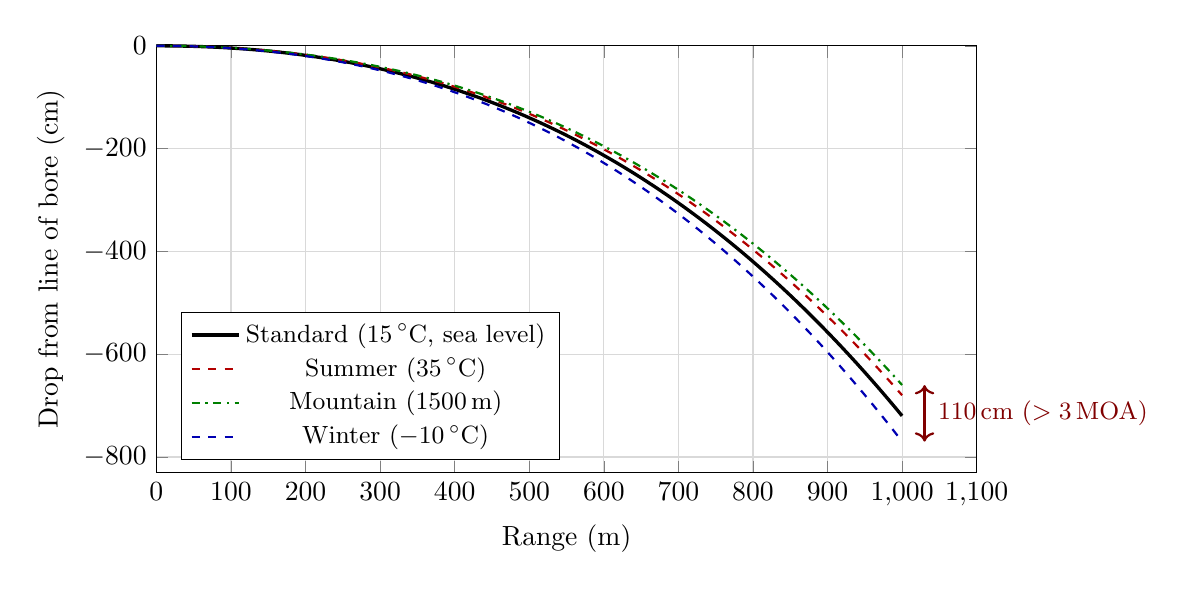
\begin{tikzpicture}
\begin{axis}[
    width=12cm, height=7cm,
    xlabel={Range (m)},
    ylabel={Drop from line of bore (cm)},
    xmin=0, xmax=1100,
    ymin=-830, ymax=0,
    grid=both,
    grid style={gray!30},
    legend pos=south west,
    legend style={font=\small},
    clip=false,
]
\addplot[very thick, black, domain=0:1000, samples=100]
    {-0.0004*x^2 - 3.2e-7*x^3};
\addlegendentry{Standard (15\,$^\circ$C, sea level)}
\addplot[thick, red!70!black, dashed, domain=0:1000, samples=100]
    {0.9444*(-0.0004*x^2 - 3.2e-7*x^3)};
\addlegendentry{Summer (35\,$^\circ$C)}
\addplot[thick, green!50!black, dashdotted, domain=0:1000, samples=100]
    {0.9167*(-0.0004*x^2 - 3.2e-7*x^3)};
\addlegendentry{Mountain (1500\,m)}
\addplot[thick, blue!70!black, dashed, domain=0:1000, samples=100]
    {1.0694*(-0.0004*x^2 - 3.2e-7*x^3)};
\addlegendentry{Winter ($-$10\,$^\circ$C)}
\draw[<->, thick, red!50!black] (axis cs:1030,-660) -- (axis cs:1030,-770);
\node[right, font=\small, text=red!50!black] at (axis cs:1035,-715) {110\,cm ($> 3$\,MOA)};
\end{axis}
\end{tikzpicture}
\caption{Schematic trajectory comparison for a 6.5\,mm 140\,gr VLD bullet ($B_C = 0.311$ G7, $v_0 = 2700$~fps) under different atmospheric conditions. The spread between extreme conditions exceeds 1~m at 1000~m ($> 3$~MOA), demonstrating the necessity of atmospheric corrections for long-range shooting. Curves are polynomial approximations scaled by density ratio.}
\label{fig:traj_atmosphere}
\end{figure}

\section{Julia Implementation: Atmospheric Model}

\begin{lstlisting}[caption={Atmospheric model in Julia},label={lst:atmos}]
# See CompetitionBallistics.jl, module Atmosphere
# Key functions:
#   std_temperature(h)           -> T [K]
#   std_pressure(h)              -> P [Pa]
#   air_density(; P, T, H)       -> rho [kg/m^3]
#   speed_of_sound(T)            -> a [m/s]
#   density_altitude(rho)        -> DA [m]
#   saturation_vapor_pressure(T) -> e_s [Pa]
\end{lstlisting}


% ============================================================================
\chapter{Interior Ballistics}
\label{ch:interior}

\section{Motivation: The Engine of the Bullet}

Before a bullet can fight the wind or drop over a thousand yards, it must be launched. Interior ballistics is the study of what happens inside the rifle's chamber and barrel from the moment the firing pin strikes the primer until the bullet exits the muzzle. It governs the brutal and violent conversion of chemical energy stored in the gunpowder (propellant) into the kinetic energy of the projectile.

For the competition shooter, interior ballistics dictates the two most important initial conditions of any shot:
\begin{enumerate}
    \item \textbf{Muzzle Velocity ($v_0$)}: The speed at which the bullet leaves the barrel.
    \item \textbf{Consistency (SD and ES)}: The Standard Deviation and Extreme Spread of that velocity across multiple shots. A high extreme spread guarantees vertical stringing (missing high or low) at extended ranges, rendering all exterior ballistic math mathematically pointless.
\end{enumerate}

To understand how a cartridge achieves a specific muzzle velocity, we must treat the rifle chamber as a high-pressure thermodynamic engine.

\paragraph{Online implementation (note).} A web implementation of the 0D model below (a Gordon's Reloading Tool--style solver) is available on Tireur.org. It is intended strictly as an \emph{educational} tool: validation against published manufacturer data shows that it currently \emph{under-predicts} both peak pressure and muzzle velocity, so it should be used to study trends---not for absolute load development \citep{grt_manual}. Always verify any charge against official manufacturer data.

\begin{figure}[H]
\centering
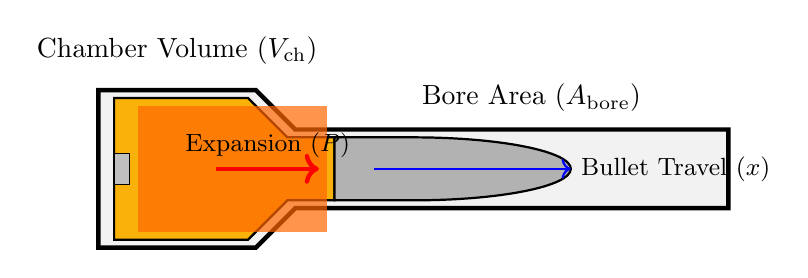
\begin{tikzpicture}
  % Barrel and Chamber outline
  \draw[ultra thick, fill=gray!10] (0, 1) -- (2, 1) -- (2.5, 0.5) -- (8, 0.5) -- (8, -0.5) -- (2.5, -0.5) -- (2, -1) -- (0, -1) -- cycle;
  % Brass Case
  \draw[thick, fill=yellow!40!orange] (0.2, 0.9) -- (1.9, 0.9) -- (2.4, 0.4) -- (3, 0.4) -- (3, -0.4) -- (2.4, -0.4) -- (1.9, -0.9) -- (0.2, -0.9) -- cycle;
  % Primer
  \draw[fill=gray!50] (0.2, 0.2) rectangle (0.4, -0.2);
  % Propellant gas/fire
  \fill[red!60!yellow, opacity=0.7] (0.5, 0.8) rectangle (2.9, -0.8);
  % Bullet
  \draw[thick, fill=gray!60] (3, 0.4) -- (4, 0.4) arc (90:-90:2 and 0.4) -- (3, -0.4) -- cycle;
  % Vectors and annotations
  \draw[->, ultra thick, red] (1.5, 0) -- (2.8, 0) node[midway, above, font=\small, text=black] {Expansion ($P$)};
  \draw[->, thick, blue] (3.5, 0) -- (6, 0) node[right, font=\small, text=black] {Bullet Travel ($x$)};
  
  \node[above] at (1, 1.2) {Chamber Volume ($V_{\mathrm{ch}}$)};
  \node[above] at (5.5, 0.6) {Bore Area ($A_{\mathrm{bore}}$)};
\end{tikzpicture}
\caption{The thermodynamic system of a rifle cartridge. Expanding gases from burning propellant create immense pressure $P$ that forces the bullet down the bore.}
\label{fig:interior_chamber}
\end{figure}

\section{The Thermodynamic Problem}

\subsection{Noble--Abel Equation of State}

When gunpowder burns, it creates gas. At the extreme pressures found in a rifle chamber (often exceeding 60,000 PSI or 400 MPa), these gases are packed so tightly that they deviate significantly from the "ideal gas" behavior taught in high school physics ($PV = nRT$). The gas molecules themselves take up physical space!

To account for this, we use the Noble--Abel equation \citep{corner1950interior,carlucci2007ballistics}, which introduces an "excluded volume" or co-volume:
\begin{equation}
  P\,(V - \eta) = n\,R_u\,T_g
  \label{eq:nobel_abel}
\end{equation}

Let's define these variables:
\begin{itemize}[noitemsep]
    \item $P$: The chamber pressure of the expanding gas.
    \item $V$: The total volume available for the gas to occupy (chamber volume plus barrel volume behind the bullet).
    \item $\eta$ (eta): The total co-volume, representing the physical space the gas molecules occupy ($\eta = n \cdot b$).
    \item $n$: The number of moles of gas produced.
    \item $R_u$: The universal gas constant ($\SI{8.3145}{\joule\per\mole\per\kelvin}$).
    \item $T_g$: The absolute temperature of the propellant gas.
\end{itemize}

By subtracting the co-volume $\eta$ from the total volume $V$, the Noble-Abel equation prevents the gas pressure from inaccurately dropping to zero.

\subsection{Energy Balance}

The first law of thermodynamics applied to the propellant--projectile system:
\begin{equation}
  Q_{\mathrm{prop}} = E_k + E_{\mathrm{heat}} + E_{\mathrm{friction}} + E_{\mathrm{gas\,KE}} + E_{\mathrm{residual}}
  \label{eq:energy_balance}
\end{equation}

The total chemical energy released by the propellant charge:
\begin{equation}
  Q_{\mathrm{prop}} = C \cdot f \cdot z
  \label{eq:Q_prop}
\end{equation}
where $C$ is the charge mass, $f$ is the impetus (force constant, energy per unit mass), and $z$ is the fraction of charge burned ($0 \le z \le 1$).

\section{Simplified Closed-Bomb Model}

In a closed bomb (no projectile motion), the pressure is:
\begin{equation}
  P = \frac{C\,f\,z}{V_{\mathrm{ch}} - C\,(1-z)/\rho_p - C\,z\,\eta_{\mathrm{sp}}}
  \label{eq:closed_bomb}
\end{equation}
where $V_{\mathrm{ch}}$ is the chamber volume, $\rho_p$ is the solid propellant density, and $\eta_{\mathrm{sp}}$ is the specific co-volume.

\section{Burn Rate Law}

The rate of gas generation follows a geometric burn rate law. For a single-perforated cylindrical grain:
\begin{equation}
  \frac{\dd z}{\dd t} = \frac{S(z)}{V_g(z)}\,\beta\,P^n
  \label{eq:burn_rate}
\end{equation}

For small arms propellants, the empirical Vieille law \citep{corner1950interior} is commonly used:
\begin{equation}
  r_b = \beta\,P^n
  \label{eq:vielle}
\end{equation}
where $r_b$ is the linear regression rate (\si{\meter\per\second}), and typical values are $n \approx 0.6$--$0.9$.

\subsection{Geometric Form Function}

For common grain geometries, the fraction burned $z$ relates to the linear fraction burned $\xi = e/e_0$ through a form function:
\begin{equation}
  z(\xi) = \xi\,(1 + \theta\,\xi)
  \label{eq:form_function}
\end{equation}
where $\theta$ is the form factor: $\theta = 0$ for a slab, $\theta > 0$ for progressive, and $\theta < 0$ for degressive grains.

\paragraph{Note on software models.} Production tools such as GRT and QuickLOAD extend this classical framework with proprietary, calibrated sub-models---notably a multi-stage form function (three stages in GRT versus two in QuickLOAD) and detailed energy-loss and effective-mass (Lagrange/Sebert) terms---fitted to closed-bomb and ballistic measurements \citep{corner1950interior,kneubuehl_ballistik,grt_manual,anderson1987ibhvg2}. These calibrated internals are not fully published; the equations above are the open, literature-based formulation.

\section{Le Duc Velocity Model}

A classical approximation for muzzle velocity useful for handloading estimates \citep{mccoy1999modern}:
\begin{equation}
  v(x) = \frac{a\,x}{b + x}
  \label{eq:leduc}
\end{equation}
where $x$ is the projectile travel distance from the cartridge case mouth, and $a$ and $b$ are empirically determined constants. As $x \to \infty$, $v \to a$, so $a$ represents the theoretical maximum velocity.

\section{Pressure--Travel Relationship}

The pressure as a function of bullet travel $x$ in the barrel:
\begin{equation}
  P(x) = \frac{m_e}{A_{\mathrm{bore}}}\,\frac{\dd v}{\dd t}
  = \frac{m_e\,v}{A_{\mathrm{bore}}}\,\frac{\dd v}{\dd x}
  \label{eq:pressure_travel}
\end{equation}
where $m_e = m + C/3$ is the effective mass and $A_{\mathrm{bore}} = \pi d^2/4$ is the bore cross-sectional area.

Using the Le Duc model, the pressure becomes:
\begin{equation}
  P(x) = \frac{m_e\,a^2\,b\,x}{A_{\mathrm{bore}}\,(b+x)^3}
  \label{eq:pressure_leduc}
\end{equation}

The peak pressure occurs at $x_{\max} = b/2$:
\begin{equation}
  P_{\max} = \frac{4\,m_e\,a^2}{27\,A_{\mathrm{bore}}\,b}
  \label{eq:peak_pressure}
\end{equation}

\section{Muzzle Velocity Estimation for Handloaders}

A practical empirical formula due to Powley and refined by \citet{litz2011applied}:
\begin{equation}
  v_0 \approx v_{\mathrm{ref}}\left(\frac{L_{\mathrm{barrel}}}{L_{\mathrm{ref}}}\right)^{0.25 \text{ to } 0.30}
  \label{eq:barrel_length_correction}
\end{equation}

A rough rule of thumb: each inch of barrel length change alters muzzle velocity by approximately \SI{20}{\fps} to \SI{35}{\fps} for typical rifle cartridges \citep{litz2011applied}.

As a practical validation of Eq.~\eqref{eq:barrel_length_correction}, consider measured data for the .308~Winchester with Lapua 155\,gr Scenar ammunition:

\begin{table}[H]
\centering
\caption{Measured muzzle velocity vs.\ barrel length, .308~Win / Lapua 155\,gr Scenar}
\label{tab:barrel_length_308}
\small
\begin{tabular}{@{}ccc@{}}
\toprule
\textbf{Barrel length (in)} & \textbf{$v_0$ (m/s)} & \textbf{$v_0$ (fps)} \\
\midrule
20 & 820 & 2690 \\
24 & 845 & 2772 \\
26 & 860 & 2822 \\
\bottomrule
\end{tabular}
\end{table}

This yields approximately \SI{12}{\meter\per\second} ($\approx$\SI{40}{\fps}) per additional inch beyond 20~inches, which is consistent with the power-law exponent of $0.27$ used in the companion Julia library. Note that the gain per inch diminishes with longer barrels, as the propellant gas expansion cools and pressure drops.

\subsection{Temperature Sensitivity of Muzzle Velocity}

Propellant burn rate is temperature-dependent. The temperature coefficient:
\begin{equation}
  \frac{\Delta v_0}{v_0} = \sigma_T\,\Delta T
  \label{eq:temp_sensitivity}
\end{equation}
where $\sigma_T$ is the temperature sensitivity coefficient, typically $0.5$ to $2.0\;\text{fps}/\degF$ ($0.9$ to $3.6\;\text{fps}/\degC$) depending on propellant. Modern temperature-stable propellants like Hodgdon Extreme series have $\sigma_T \approx 0.5\;\text{fps}/\degF$ ($0.9\;\text{fps}/\degC$) \citep{litz2011applied}.

\default{$\sigma_T = 1.0\;\text{fps}/\degF = 1.8\;\text{fps}/\degC$}


% ============================================================================
\chapter{Transitional Ballistics}
\label{ch:transitional}

\section{Motivation: The Chaos of the Muzzle}

Transitional (or intermediate) ballistics covers the violent and chaotic fraction of a millisecond between interior ballistics (the barrel) and exterior ballistics (free flight). It represents the exact moment the bullet exits the protective confinement of the muzzle and punches into the atmosphere.

Why does a shooter care about this microsecond? Because this is where the bullet is most vulnerable. A perfectly loaded cartridge and a perfectly aimed rifle can be completely ruined by a bad muzzle crown or inconsistent gas release, which will instantly destabilize the bullet before its flight even begins. 

\section{Muzzle Gas Dynamics}

When the bullet finally unplugs the barrel, the high-pressure propellant gases (still trapped behind the bullet at pressures of \SI{10}{}--\SI{70}{\mega\pascal}) suddenly vent into the atmosphere. Because these gases are incredibly hot and highly pressurized, they expand outward at velocities \emph{faster} than the bullet itself. The bullet is essentially blasted from behind by its own exhaust.

This creates a complex and turbulent shock-wave structure just inches in front of the muzzle \citep{carlucci2007ballistics}:

\begin{figure}[H]
\centering
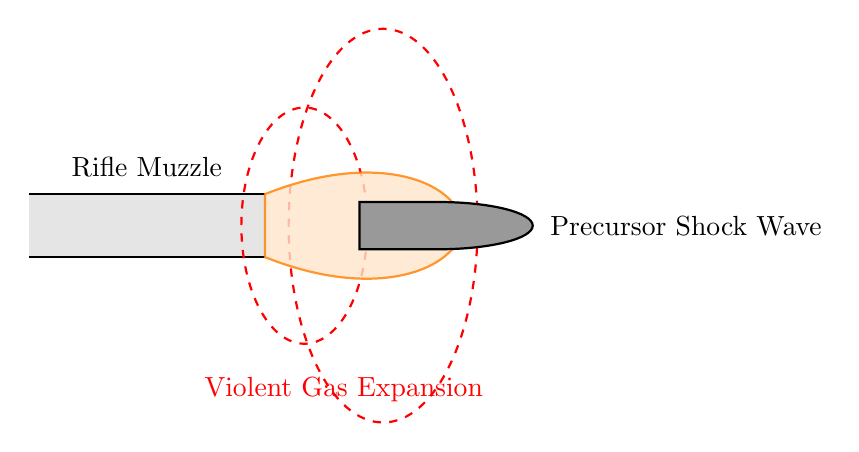
\begin{tikzpicture}
  % Barrel
  \fill[gray!20] (-3, 0.4) rectangle (0, -0.4);
  \draw[thick] (-3, 0.4) -- (0, 0.4);
  \draw[thick] (-3, -0.4) -- (0, -0.4);
  
  % Expanding gases
  \draw[red, dashed, thick] (0.5, 0) ellipse (0.8 and 1.5);
  \draw[red, dashed, thick] (1.5, 0) ellipse (1.2 and 2.5);
  
  % Mach disk / bottle shock
  \draw[orange, thick, fill=orange!20, opacity=0.8] (0, 0.4) .. controls (1.5, 1) and (2.5, 0.5) .. (2.5, 0) 
  .. controls (2.5, -0.5) and (1.5, -1) .. (0, -0.4) -- cycle;
  
  % Bullet
  \draw[fill=gray!80, thick] (1.2, 0.3) -- (2.2, 0.3) arc(90:-90:1.2 and 0.3) -- (1.2, -0.3) -- cycle;
  
  % Text annotations
  \node[above] at (-1.5, 0.5) {Rifle Muzzle};
  \node[right] at (3.5, 0) {Precursor Shock Wave};
  \node[below, text=red] at (1, -1.8) {Violent Gas Expansion};
\end{tikzpicture}
\caption{Transitional ballistics: The bullet exiting the muzzle gets overtaken by rapidly expanding, supersonic propellant gases. A symmetrical gas release here is paramount to accuracy.}
\label{fig:muzzle_gas}
\end{figure}

The structure consists of:
\begin{enumerate}
  \item \textbf{Muzzle blast wave}: A spherical shock radiating outward (the "bang" you hear).
  \item \textbf{Precursor blast}: Produced from the column of air that was compressed ahead of the bullet inside the barrel.
  \item \textbf{Bottle shock}: The characteristic diamond-pattern Mach disk structure formed by the underexpanded supersonic gas jet accelerating past the bullet.
\end{enumerate}

\section{Muzzle Tip-Off and Initial Yaw}

The concept of "tip-off" is critical. If the muzzle crown is damaged, or if the bullet's base is not perfectly square, the escaping gases will vent asymmetrically. 

Let's define the variables for this instability:
\begin{itemize}[noitemsep]
    \item $\omega$ (omega): The angular velocity or "tip-off rate" imparted to the bullet (\si{\radian\per\second}).
    \item $\alpha_0$ (alpha zero): The initial yaw angle of the bullet as it exits the muzzle (degrees).
\end{itemize}

Asymmetric gas forces impart a small angular velocity ($\omega$). The resulting initial yaw angle $\alpha_0$ is typically small ($0.5^\circ$--$3^\circ$) for match-grade ammunition. However, any yaw at the muzzle drastically increases early aerodynamic drag and causes the bullet to precess (wobble) in flight, opening up group sizes.

\section{Base Drag Transition}

Inside the barrel, the base of the bullet is pushed forward by thousands of PSI of pressure. The moment it exits, this high pressure rapidly drops to the ambient atmospheric pressure, creating a sudden vacuum effect behind the bullet. This causes \emph{base drag} to increase significantly, transitioning from a suppressed value to its full free-flight aerodynamic penalty over a distance of approximately 5--20 calibers from the muzzle \citep{mccoy1999modern}.

\section{Crown Effects}

Because of this violent gas transition, the muzzle crown (the final machined edge at the barrel's exit) is one of the most critical parts of the rifle. It must be perfectly concentric and perpendicular to the bore axis to ensure gases release symmetrically around the entire circumference of the bullet base at the exact same microsecond.


% ============================================================================
\chapter{Exterior Ballistics: Core Theory}
\label{ch:exterior}

\section{Motivation: The Math of Free Flight}

Once the bullet escapes the muzzle, all active propulsion ceases. The projectile enters "free flight." From this point until it strikes the target, the bullet's path is entirely at the mercy of classical physics. Exterior ballistics is the mathematical prediction of this flight path. For a competitive shooter, this is the core of their craft: translating the laws of physics into correct scope dial adjustments.

To predict where a bullet will land, we must solve equations of motion that account for two primary forces:
\begin{enumerate}
    \item \textbf{Gravity}: Continually accelerating the bullet toward the earth, determining "drop."
    \item \textbf{Aerodynamic Drag}: The immense friction of the air, rapidly bleeding off the bullet's velocity and magnifying the time gravity has to act.
\end{enumerate}

\section{Vacuum Trajectory (The Baseline)}

Before conquering air resistance, we must understand the baseline system. In a perfect vacuum (ignoring air resistance), the trajectory is a simple parabola. While this model is \emph{useless for real-world rifle ballistics} (because supersonic drag dominates behavior), it serves as a mathematical foundation. 

Let's define the fundamental launch parameters:
\begin{itemize}[noitemsep]
    \item $t$: Time elapsed since the bullet left the muzzle (seconds, \si{\second}).
    \item $v_0$: Initial muzzle velocity (e.g., \si{\meter\per\second} or \si{\fps}).
    \item $\theta$ (theta): The launch elevation angle, or "look-up" angle of the barrel relative to the horizontal.
    \item $g$: Standard gravitational acceleration (\SI{9.80665}{\meter\per\second\squared}).
    \item $x(t)$: The horizontal distance traveled at time $t$.
    \item $y(t)$: The vertical height of the bullet at time $t$.
\end{itemize}

Using basic Newtonian mechanics, the parametric equations of motion in a vacuum are:
\begin{align}
  x(t) &= v_0 \cos\theta \cdot t \label{eq:vac_x}\\
  y(t) &= v_0 \sin\theta \cdot t - \frac{1}{2}g\,t^2 \label{eq:vac_y}
\end{align}

Eliminating time $t$ from Eq.~\eqref{eq:vac_x} and substituting it into Eq.~\eqref{eq:vac_y} yields the single continuous trajectory equation in terms of horizontal distance $x$:
\begin{equation}
  \boxed{y(x) = x \tan\theta - \frac{g x^2}{2 v_0^2 \cos^2\theta}}
  \label{eq:vac_y_x}
\end{equation}

The range in vacuum:
\begin{equation}
  R_{\mathrm{vac}} = \frac{v_0^2 \sin 2\theta}{g}
  \label{eq:vac_range}
\end{equation}

\section{Aerodynamic Drag}

\subsection{The Drag Equation}

The aerodynamic drag force opposes the bullet's motion through the air:
\begin{equation}
  \boxed{F_D = \frac{1}{2}\,\rho\,v^2\,\Cd(\Mach)\,A}
  \label{eq:drag_force}
\end{equation}

The drag deceleration:
\begin{equation}
  a_D = \frac{F_D}{m} = \frac{\rho\,v^2\,\Cd\,A}{2\,m}
  \label{eq:drag_decel}
\end{equation}

\subsection{Drag Coefficient and Mach Number}

The drag coefficient $\Cd$ is fundamentally a function of Mach number $\Mach = v/a$, Reynolds number $\Rey$, and projectile geometry. For small-arms bullets, $\Rey$ effects are secondary, and $\Cd$ is treated as a function of $\Mach$ alone \citep{mccoy1999modern}.

The $\Cd$--$\Mach$ curve has characteristic regimes: subsonic ($\Mach < 0.8$) with low, slowly varying $\Cd$; transonic ($0.8 < \Mach < 1.2$) with a sharp rise; and supersonic ($\Mach > 1.2$) with gradually decreasing $\Cd$.

\begin{figure}[H]
\centering
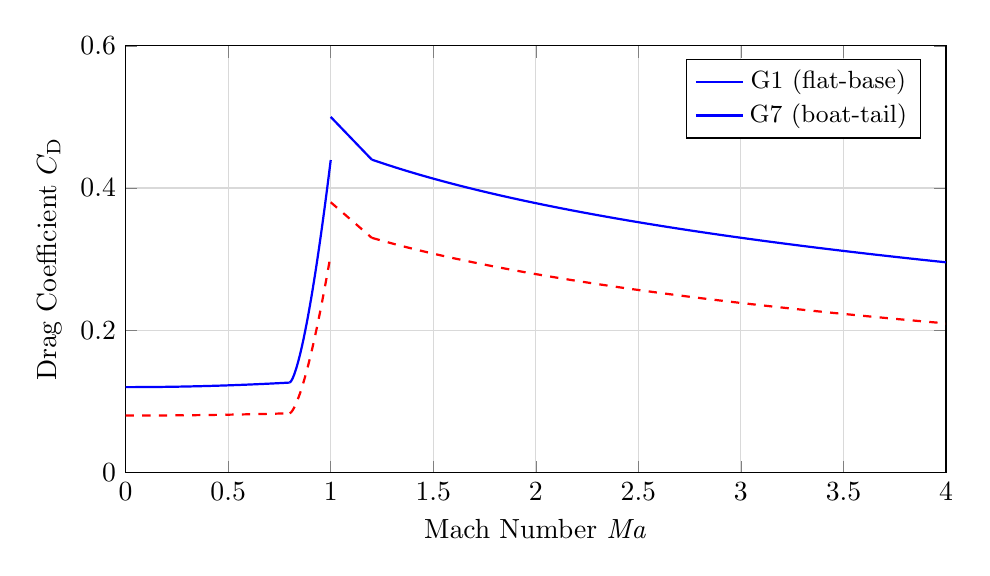
\begin{tikzpicture}
\begin{axis}[
    width=12cm, height=7cm,
    xlabel={Mach Number $\Mach$},
    ylabel={Drag Coefficient $\Cd$},
    xmin=0, xmax=4.0,
    ymin=0, ymax=0.6,
    grid=both,
    grid style={gray!30},
    legend pos=north east,
    legend style={font=\small},
]
\addplot[thick, blue, domain=0:0.8, samples=30] {0.12 + 0.01*x^2};
\addplot[thick, blue, domain=0.8:1.0, samples=30] {0.12 + 0.01*0.64 + 3.5*(x-0.8)^1.5};
\addplot[thick, blue, domain=1.0:1.2, samples=30] {0.50 - 0.3*(x-1.0)};
\addplot[thick, blue, domain=1.2:4.0, samples=50] {0.44 - 0.12*ln(x/1.2)};
\addplot[thick, red, dashed, domain=0:0.8, samples=30] {0.08 + 0.005*x^2};
\addplot[thick, red, dashed, domain=0.8:1.0, samples=30] {0.08 + 0.005*0.64 + 2.5*(x-0.8)^1.5};
\addplot[thick, red, dashed, domain=1.0:1.2, samples=30] {0.38 - 0.25*(x-1.0)};
\addplot[thick, red, dashed, domain=1.2:4.0, samples=50] {0.33 - 0.10*ln(x/1.2)};
\legend{G1 (flat-base), G7 (boat-tail)}
\end{axis}
\end{tikzpicture}
\caption{Schematic drag coefficient vs.\ Mach number for G1 and G7 reference projectiles.}
\label{fig:cd_mach}
\end{figure}

\subsection{Analytical Solution for 1D Drag}

While modern ballistics requires numerical integration (see Section~\ref{sec:numerical}), a simplified 1D model where $\Cd$ is assumed constant provides useful insights into the scaling of range and velocity with respect to the ballistic coefficient.

Consider purely horizontal motion with drag as the only force:
\begin{equation}
  \frac{\dd v}{\dd t} = -k\,v^2, \quad \text{where } k = \frac{\rho\,\Cd\,A}{2\,m}
  \label{eq:1d_drag_ode}
\end{equation}

Separating variables and integrating:
\begin{equation}
  \int_{v_0}^{v} \frac{\dd v'}{(v')^2} = -k \int_{0}^{t} \dd t' \implies -\left[\frac{1}{v'}\right]_{v_0}^{v} = -k\,t
\end{equation}

The velocity as a function of time is:
\begin{equation}
  \boxed{v(t) = \frac{v_0}{1 + k\,v_0\,t}}
  \label{eq:1d_v_t}
\end{equation}

Integrating once more to find the distance $x(t)$:
\begin{equation}
  x(t) = \int_{0}^{t} \frac{v_0}{1 + k\,v_0\,t'} \dd t' = \frac{1}{k} \ln(1 + k\,v_0\,t)
\end{equation}

Solving for $t$ in terms of $x$:
\begin{equation}
  t = \frac{e^{kx} - 1}{k\,v_0}
\end{equation}

Substituting this into Eq.~\eqref{eq:1d_v_t} yields the velocity as a function of distance:
\begin{equation}
  \boxed{v(x) = v_0 e^{-kx}}
  \label{eq:1d_v_x}
\end{equation}

This exponential decay demonstrates how the "Physics BC" (contained within $k$) determines the velocity retention of the projectile.

\section{Ballistic Coefficient}
\label{sec:bc}

The ballistic coefficient $\Bc$ is defined as:
\begin{equation}
  \boxed{\Bc = \frac{\sd}{i} = \frac{m}{i\,d^2}}
  \label{eq:bc_definition}
\end{equation}
where $\sd = m/d^2$ is the sectional density and $i$ is the form factor:
\begin{equation}
  i(\Mach) = \frac{\Cd^{\mathrm{bullet}}(\Mach)}{\Cd^{\mathrm{std}}(\Mach)}
  \label{eq:form_factor}
\end{equation}

$\Bc$ is only meaningful when referenced to a specific drag model (G1, G7, etc.).

\subsection{Standard Conditions for BC}

By convention, $\Bc$ values are quoted at standard atmosphere conditions. To use $\Bc$ at non-standard conditions:
\begin{equation}
  {B_C}_{\mathrm{actual}} = {B_C}_{\mathrm{std}} \cdot \frac{\rho_0}{\rho_{\mathrm{actual}}}
  \label{eq:bc_density_correction}
\end{equation}

\section{Standard Drag Models (G1 through G8)}
\label{sec:drag_models}

\begin{table}[H]
\centering
\caption{BRL Standard Drag Models \citep{mccoy1999modern, ingalls1893exterior}}
\label{tab:drag_models}
\begin{tabularx}{\textwidth}{@{}lXl@{}}
\toprule
\textbf{Model} & \textbf{Reference Projectile Shape} & \textbf{Primary Use} \\
\midrule
G1 & Flat-base with 2-caliber ogive nose & Traditional default; hunting bullets \\
G7 & Long, secant-ogive, boat-tail & \textbf{Best for modern VLD match bullets} \\
G8 & Similar to G7 with flat base & Flat-base match bullets \\
GL & Blunt-nose lead bullet & Cast lead bullets \\
\bottomrule
\end{tabularx}
\end{table}

\begin{figure}[H]
\centering
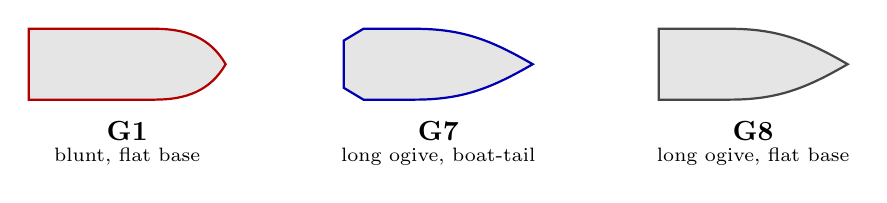
\begin{tikzpicture}[every node/.style={font=\small}]
  % G1 : blunt, flat base
  \fill[gray!20, draw=red!70!black, thick]
    (0,0.45) -- (1.6,0.45) to[out=0,in=120] (2.5,0) to[out=-120,in=0] (1.6,-0.45) -- (0,-0.45) -- cycle;
  \node[font=\bfseries] at (1.25,-0.85) {G1};
  \node[font=\scriptsize] at (1.25,-1.18) {blunt, flat base};
  % G7 : long secant ogive, boat-tail
  \fill[gray!20, draw=blue!70!black, thick]
    (4.0,0.30) -- (4.25,0.45) -- (4.9,0.45) to[out=0,in=150] (6.4,0) to[out=-150,in=0] (4.9,-0.45) -- (4.25,-0.45) -- (4.0,-0.30) -- cycle;
  \node[font=\bfseries] at (5.2,-0.85) {G7};
  \node[font=\scriptsize] at (5.2,-1.18) {long ogive, boat-tail};
  % G8 : long secant ogive, flat base
  \fill[gray!20, draw=gray!55!black, thick]
    (8.0,0.45) -- (8.9,0.45) to[out=0,in=150] (10.4,0) to[out=-150,in=0] (8.9,-0.45) -- (8.0,-0.45) -- cycle;
  \node[font=\bfseries] at (9.2,-0.85) {G8};
  \node[font=\scriptsize] at (9.2,-1.18) {long ogive, flat base};
\end{tikzpicture}
\caption{Schematic silhouettes of three reference projectiles (nose to the right). The blunt, flat-based G1 differs markedly from a modern match bullet, whereas the long boat-tailed G7 closely matches it; G8 shares the G7 nose but keeps a flat base.}
\label{fig:drag_shapes}
\end{figure}

\textbf{For competition rifle shooting, G7 is strongly preferred} over G1 for modern VLD boat-tail bullets because the G7 reference shape more closely matches these bullets, resulting in a form factor $i$ closer to 1.0 and a more constant $\Bc$ across the velocity range \citep{litz2011applied}.

\begin{figure}[H]
\centering
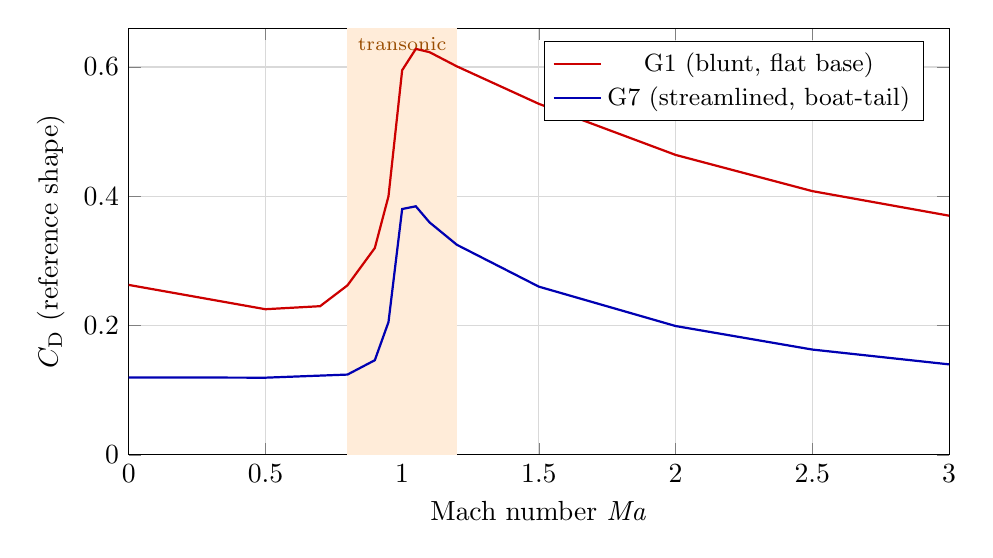
\begin{tikzpicture}
\begin{axis}[
    width=12cm, height=7cm,
    xlabel={Mach number $\Mach$},
    ylabel={$\Cd$ (reference shape)},
    xmin=0, xmax=3, ymin=0, ymax=0.66,
    grid=both, grid style={gray!30},
    legend pos=north east, legend style={font=\small},
    xtick={0,0.5,1,1.5,2,2.5,3},
]
\fill[orange!15] (axis cs:0.8,0) rectangle (axis cs:1.2,0.66);
\node[font=\scriptsize, orange!60!black] at (axis cs:1.0,0.635) {transonic};
\addplot[thick, red!80!black] coordinates {
  (0,0.2629)(0.5,0.2253)(0.7,0.2300)(0.8,0.2622)(0.9,0.3200)(0.95,0.4000)
  (1.0,0.5950)(1.05,0.6280)(1.1,0.6230)(1.2,0.6010)(1.5,0.5430)
  (2.0,0.4640)(2.5,0.4080)(3.0,0.3700)};
\addlegendentry{G1 (blunt, flat base)}
\addplot[thick, blue!70!black] coordinates {
  (0,0.1198)(0.5,0.1194)(0.8,0.1242)(0.9,0.1464)(0.95,0.2054)
  (1.0,0.3803)(1.05,0.3845)(1.1,0.3597)(1.2,0.3250)(1.5,0.2602)
  (2.0,0.1993)(2.5,0.1629)(3.0,0.1400)};
\addlegendentry{G7 (streamlined, boat-tail)}
\end{axis}
\end{tikzpicture}
\caption{Drag coefficient of the G1 and G7 reference shapes versus Mach number (G7 values from Table~\ref{tab:g7_values}; G1 representative BRL data). Both rise sharply through the transonic region, but the slender G7 has a markedly lower, flatter peak---the physical reason its $\Bc$ stays nearly constant across the supersonic range.}
\label{fig:cd_mach_compare}
\end{figure}

\subsection{G7 Drag Function}

\begin{table}[H]
\centering
\caption{Selected G7 drag coefficient values \citep{mccoy1999modern}}
\label{tab:g7_values}
\begin{tabular}{@{}rr@{\qquad}rr@{\qquad}rr@{}}
\toprule
$\Mach$ & $\Cd^{\mathrm{G7}}$ & $\Mach$ & $\Cd^{\mathrm{G7}}$ & $\Mach$ & $\Cd^{\mathrm{G7}}$ \\
\midrule
0.00 & 0.1198 & 1.00 & 0.3803 & 2.00 & 0.1993 \\
0.50 & 0.1194 & 1.05 & 0.3845 & 2.50 & 0.1629 \\
0.80 & 0.1242 & 1.10 & 0.3597 & 3.00 & 0.1400 \\
0.90 & 0.1464 & 1.20 & 0.3250 & 3.50 & 0.1225 \\
0.95 & 0.2054 & 1.50 & 0.2602 & 4.00 & 0.1090 \\
\bottomrule
\end{tabular}
\end{table}

The values above are reproduced verbatim from the table embedded in the solver
(\texttt{G7\_RAW} in \texttt{CompetitionBallistics.js}); the solver interpolates
this same data at run time, so the documentation and the implementation are
guaranteed to agree.

\subsection{Drag Functions vs.\ Siacci Tables: a Common Confusion}

\noindent
The $\Cd(\Mach)$ tables (G1, G7, \dots) are \emph{aerodynamic} data: $\Cd$ is
dimensionless and depends only on the projectile geometry and the Mach number,
\emph{not} on the atmosphere. They are therefore identical whether one takes them
from McCoy~\citep{mccoy1999modern} or from a tabulation such as JBM's. The
atmosphere only enters our solver through the \emph{actual} air density $\rho$ and
speed of sound $a(T)$, both recomputed from the ICAO model
(\S\ref{sec:icao}) at every step via
$D = \tfrac{1}{2}\rho\,\Cd(\Mach)\,A\,i/m$, with $i = \sd/\Bc$ the form factor.

What \emph{does} depend on the standard atmosphere are the integrated
\emph{Siacci tables} $S(V), A(V), I(V), T(V)$, because their integration
involves the standard density and speed of sound. This is the well-known caveat
that Siacci tables computed under the ICAO atmosphere differ from those in
McCoy's book. \textbf{Our solver uses no Siacci table}---it integrates the 3-DOF
equations numerically---so this caveat does not apply here.

The single genuine consistency requirement is that the user-supplied $\Bc$ be
referenced to the same standard atmosphere as the code, namely ICAO
($\rho_0 = \SI{1.225}{\kilogram\per\meter\cubed}$, \SI{15}{\celsius}, dry).
Modern G7 values (Berger, Hornady, Litz/Applied Ballistics) are all
ICAO-referenced. Older \emph{Army Standard Metro} (ASM) $\Bc$ values
(\SI{29.53}{inHg}, 78\,\% RH) carry a $\approx 0.4$--$0.5\,\%$ density offset.

\paragraph{Warning on Legacy Calculators (e.g., JBM):} Many legacy ballistic calculators, such as JBM Ballistics, enable the Army Standard Metro atmosphere by default. If a modern ICAO-referenced G7 BC is input into an ASM-default calculator without explicitly disabling the Metro setting, the solver will silently apply a density offset. Because ASM air is lighter than ICAO air, this introduces an artificial trajectory error that grows significantly at extended ranges. The \texttt{CompetitionBallistics} engine exclusively uses the modern ICAO standard, ensuring native 1:1 compatibility with all contemporary manufacturer BCs without requiring any error-prone conversions.

\section{Doppler Radar Drag Measurement}
\label{sec:doppler}

The drag coefficient tables (G1, G7, etc.) originate from experimental measurements. The modern gold standard is \emph{Doppler radar tracking}, which has largely superseded earlier spark-range and yaw-card methods \citep{mccoy1999modern, braun1958aerodynamic}.

\subsection{Measurement Principle}

A continuous-wave (CW) Doppler radar illuminates the bullet in flight and measures the frequency shift of the reflected signal:
\begin{equation}
  f_D = \frac{2\,v\,\cos\theta_r}{\lambda}
  \label{eq:doppler_freq}
\end{equation}
where $f_D$ is the Doppler shift frequency, $v$ is the bullet velocity, $\theta_r$ is the angle between the velocity vector and the radar beam, and $\lambda$ is the radar wavelength. The velocity is sampled at rates of 1--10\,kHz, yielding a near-continuous $v(t)$ record over the entire flight.

\subsection{Extracting $\Cd(\Mach)$ from Radar Data}

From the measured velocity--time history, the drag coefficient is extracted by inverting the equation of motion. For a near-horizontal trajectory:
\begin{equation}
  \Cd(\Mach) = -\frac{2\,m}{\rho\,A\,v^2}\,\frac{\dd v}{\dd t}
  \label{eq:cd_from_radar}
\end{equation}

The derivative $\dd v/\dd t$ is computed numerically from the sampled $v(t)$ data. Since numerical differentiation amplifies noise, the raw data is first smoothed using a Savitzky--Golay filter or a cubic smoothing spline before differentiation.

The Mach number at each time step is:
\begin{equation}
  \Mach(t) = \frac{v(t)}{a\bigl(T(h(t))\bigr)}
  \label{eq:mach_from_radar}
\end{equation}
where $a$ is the local speed of sound, corrected for the altitude $h(t)$ along the trajectory.

\subsection{Advantages over Classical Methods}

Doppler radar provides the complete $\Cd(\Mach)$ curve from a \emph{single firing}, whereas spark-range methods require many shots at different velocities. This is the method used by:

\begin{itemize}[nosep]
  \item The BRL/ARL at Aberdeen Proving Ground to produce the definitive G1--G8 tables.
  \item Bryan Litz (Applied Ballistics) to measure custom drag curves for individual bullet models, published as ``CDM'' (Custom Drag Model) data \citep{litz2015ballistic}.
  \item Military proving grounds worldwide for projectile development.
\end{itemize}

The custom drag model approach bypasses the form-factor approximation entirely: instead of $\Cd = i \cdot \Cd^{\mathrm{std}}$, the actual measured $\Cd(\Mach)$ curve for the specific bullet is used directly. This eliminates the error from form-factor variation with Mach number and is the most accurate approach available.

\subsection{Interpolation of Tabular Drag Data}
\label{sec:interpolation}

Whether using the standard G1/G7 tables or a custom Doppler-derived curve, the drag coefficient must be evaluated at arbitrary Mach numbers during trajectory integration. Two interpolation methods are common:

\textbf{Linear interpolation} (used in many legacy solvers): Given tabular data $\{(\Mach_i, C_{D,i})\}$, find the bracketing interval $[\Mach_k, \Mach_{k+1}]$ and compute:
\begin{equation}
  \Cd(\Mach) = C_{D,k} + \frac{C_{D,k+1} - C_{D,k}}{\Mach_{k+1} - \Mach_k}\,(\Mach - \Mach_k)
  \label{eq:linear_interp}
\end{equation}

Linear interpolation introduces slope discontinuities at each table point. In the transonic region where $\Cd$ changes rapidly, these discontinuities can produce small but systematic trajectory errors.

\textbf{Cubic spline interpolation} (recommended): A natural cubic spline $S(\Mach)$ is fitted through all $n$ data points, producing a $C^2$-continuous curve (continuous through the second derivative). The spline on each interval $[\Mach_k, \Mach_{k+1}]$ is:
\begin{equation}
  S(\Mach) = a_k + b_k\,(\Mach - \Mach_k) + c_k\,(\Mach - \Mach_k)^2 + d_k\,(\Mach - \Mach_k)^3
  \label{eq:cubic_spline}
\end{equation}
where the coefficients $\{a_k, b_k, c_k, d_k\}$ are determined by enforcing continuity of $S$, $S'$, and $S''$ at interior knots, plus natural boundary conditions ($S'' = 0$ at endpoints). This requires solving a tridiagonal linear system of size $n$, which is $O(n)$ and needs to be done only once during initialization.

Cubic spline interpolation is particularly important in the transonic region ($0.9 < \Mach < 1.2$) where the $\Cd$ curve has its steepest gradient. The smooth derivative ensures that the drag force varies smoothly as the bullet decelerates through the sound barrier, eliminating artificial trajectory perturbations.

\subsubsection*{The spline is better only where the table is dense}

This recommendation holds for the \emph{standard} tables and must not be carried over
to sparse measured ones. A decimation test --- remove every second node, rebuild both
interpolants on what remains, and score them on the removed values, whose truth is
known --- reverses the verdict according to the sampling:

\begin{center}
\begin{tabular}{lccc}
\toprule
Table & Nodes & Linear & Spline \\
\midrule
G7 standard      & 65 & 0.099\,\% & \textbf{0.049\,\%} \\
G1 standard      & 53 & 0.424\,\% & \textbf{0.069\,\%} \\
McCoy .308 $C_{D_0}$ & 15 & \textbf{0.68\,\%} & 8.89\,\% \\
McCoy 105\,mm $C_{D_0}$ & 12 & \textbf{2.86\,\%} & 6.93\,\% \\
\bottomrule
\end{tabular}
\end{center}

The criterion is not ``spline versus linear'' but \emph{sampling density relative to
curvature}. McCoy's range-reduced tables are sparse and deliberately clustered on the
transonic knee --- his points sit at $\Mach = 0.90$, $0.95$, $1.00$, $1.05$, $1.10$,
$1.20$ --- so the steep rise imposes derivatives that the spline propagates as
oscillation into the neighbouring intervals, where it becomes up to thirteen times
worse than a straight line. The 6-DOF coefficient sets therefore read their tables
\emph{linearly}, on purpose.

The companion Julia implementation (Appendix~\ref{app:julia_file}) provides both linear and cubic spline interpolation via the \texttt{DragModels} module. Since 2026-08-14 \texttt{drag\_coefficient} defaults to the spline, matching the JavaScript port and this section; it previously defaulted to linear, in contradiction with both.

\section{Equations of Motion: 3-DOF Point-Mass Model}
\label{sec:3dof}

\subsection{Coordinate System}

We use a ground-fixed, flat-Earth coordinate system: $x$ (downrange), $y$ (vertical, upward positive), $z$ (cross-range, positive right).

\subsection{Vector Equation of Motion}

\begin{equation}
  \boxed{m\,\frac{\dd \vvec}{\dd t} = -\frac{1}{2}\,\rho\,\|\vvec_{\mathrm{rel}}\|\,\vvec_{\mathrm{rel}}\,\Cd(\Mach)\,A + m\,\gvec}
  \label{eq:3dof_vector}
\end{equation}
where $\vvec_{\mathrm{rel}} = \vvec - \vvec_{\mathrm{wind}}$ and $\gvec = (0, -g, 0)^T$.

\subsection{Scalar Component Equations}

\begin{align}
  \frac{\dd v_x}{\dd t} &= -\frac{\rho\,\Cd\,A}{2\,m}\,v_{\mathrm{rel}}\,(v_x - w_x) \label{eq:3dof_x}\\
  \frac{\dd v_y}{\dd t} &= -\frac{\rho\,\Cd\,A}{2\,m}\,v_{\mathrm{rel}}\,(v_y - w_y) - g \label{eq:3dof_y}\\
  \frac{\dd v_z}{\dd t} &= -\frac{\rho\,\Cd\,A}{2\,m}\,v_{\mathrm{rel}}\,(v_z - w_z) \label{eq:3dof_z}
\end{align}
where $v_{\mathrm{rel}} = \sqrt{(v_x-w_x)^2 + (v_y-w_y)^2 + (v_z-w_z)^2}$.

\subsection{Using the Ballistic Coefficient}

Substituting the form factor relationship $\Cd = i \cdot \Cd^{\mathrm{std}}$ and the ballistic coefficient definition $\Bc = m/(i\,d^2)$:
\begin{equation}
  \frac{\rho\,\Cd\,A}{2\,m} = \frac{\rho\,\Cd^{\mathrm{std}}\,\pi}{8\,\Bc}
  \label{eq:drag_with_bc}
\end{equation}
where $i$ is the projectile's form factor, $\Cd^{\mathrm{std}}$ is the drag coefficient of the standard projectile (G1 or G7), and $d$ is the caliber.

\section{Numerical Integration}
\label{sec:numerical}

Since the system of equations \eqref{eq:3dof_x}--\eqref{eq:3dof_z} has no closed-form solution due to the non-linear dependence of $\Cd$ on velocity, it must be solved numerically.

\subsection{Euler Method}

The simplest numerical approach is the first-order Euler method, which updates the state vector using the derivative at the beginning of each time step $\Delta t$:
\begin{align}
  v_x^{n+1} &= v_x^n + \Delta t \left(-\frac{\rho\,\Cd\,A}{2\,m}\,v^n\,(v_x^n - w_x)\right) \label{eq:euler_vx}\\
  v_y^{n+1} &= v_y^n + \Delta t \left(-\frac{\rho\,\Cd\,A}{2\,m}\,v^n\,(v_y^n - w_y) - g\right) \label{eq:euler_vy}\\
  x^{n+1} &= x^n + v_x^n\,\Delta t \label{eq:euler_x}\\
  y^{n+1} &= y^n + v_y^n\,\Delta t \label{eq:euler_y}
\end{align}
where $v^n = \sqrt{(v_x^n-w_x)^2 + (v_y^n-w_y)^2 + (v_z^n-w_z)^2}$. While intuitive and easy to implement, the Euler method requires very small time steps to maintain stability and accuracy.

\subsection{Runge--Kutta (RK4) \& Area Scaling}

Modern ballistic solvers use higher-order methods, typically the 4th-order Runge--Kutta (RK4) method, which provides a much better balance of speed and precision by sampling the derivative at multiple points within the time step \citep{press2007numerical}:
\begin{align}
  \bm{k}_1 &= h\,\bm{f}(t_n, \bm{y}_n) \\
  \bm{k}_2 &= h\,\bm{f}(t_n + h/2, \bm{y}_n + \bm{k}_1/2) \\
  \bm{k}_3 &= h\,\bm{f}(t_n + h/2, \bm{y}_n + \bm{k}_2/2) \\
  \bm{k}_4 &= h\,\bm{f}(t_n + h, \bm{y}_n + \bm{k}_3) \\
  \bm{y}_{n+1} &= \bm{y}_n + \tfrac{1}{6}(\bm{k}_1 + 2\bm{k}_2 + 2\bm{k}_3 + \bm{k}_4)
  \label{eq:rk4}
\end{align}
where $h$ is the time step, $\bm{y}_n$ is the full state vector $(x, y, z, v_x, v_y, v_z)$ at time $t_n$, and $\bm{f}$ is the vector of derivatives (velocities and accelerations).

\paragraph{Version 3.1 Mathematical Corrections:} 
It is critical to apply the RK4 integration to the \emph{full state vector} rather than decoupling position and velocity (a common error that degrades long-range accuracy). Furthermore, when scaling the reference drag by the Ballistic Coefficient ($\text{BC} = m / i d^2$), one must account for the physical area $A = \pi d^2 / 4$. Thus, the effective deceleration must be multiplied by a geometric correction factor of $4/\pi$ to bridge the shooting definition of sectional density and the physical drag force. These corrections ensure sub-MOA consistency with industry reference tools like JBM Ballistics at ranges exceeding 1,000 yards.

A typical time step of $h = \SI{0.0005}{\second}$ to $\SI{0.001}{\second}$ is sufficient.


% ============================================================================
\chapter{Exterior Ballistics: Advanced Effects}
\label{ch:advanced}

\section{Motivation: Beyond Gravity}

While gravity is a merciless absolute, it is highly predictable. A shooter simply needs a precise laser rangefinder to account for drop. The true separator of amateur and expert long-range shooters is the mastery of \emph{advanced exterior ballistics}, primarily wind deflection and gyroscopic drift.

Why is wind reading considered a dark art? Because wind is invisible, highly volatile, and acts on a bullet in a deeply counter-intuitive way. The most crucial concept in long-range shooting is realizing that wind does \emph{not} blow a bullet straight sideways like a piece of paper. Instead, wind deflection is entirely governed by how much \emph{drag} the bullet experiences. 

\section{Wind Deflection}
\label{sec:wind}

Wind is the single largest variable in long-range competition shooting.

\subsection{Wind Components (Vectors)}

Before calculating deflection, we must break the total wind vector into its forward/backward and left/right components relative to the shooter's line of sight.

Let's clearly define our variables:
\begin{itemize}[noitemsep]
    \item $W$: The absolute wind velocity (\si{\meter\per\second} or \si{\mph}).
    \item $\alpha_w$ (alpha $w$): The angle of the wind vector relative to the line of fire (e.g., $90^\circ$ is a full crosswind).
    \item $w_x$: The headwind (negative) or tailwind (positive) velocity vector.
    \item $w_z$: The lateral crosswind velocity vector.
\end{itemize}

\begin{figure}[H]
\centering
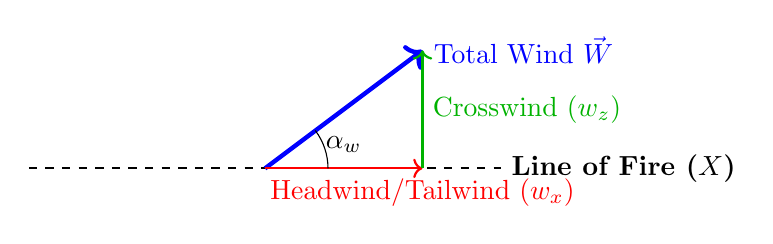
\begin{tikzpicture}
  % Shooter to Target line
  \draw[dashed, thick] (0,0) -- (6,0) node[right, font=\bfseries] {Line of Fire ($X$)};
  
  % Wind Vector
  \draw[->, ultra thick, blue] (3,0) -- (5, 1.5) node[right] {Total Wind $\vec{W}$};
  
  % Components
  \draw[->, thick, red] (3,0) -- (5,0) node[below] {Headwind/Tailwind ($w_x$)};
  \draw[->, thick, green!70!black] (5,0) -- (5, 1.5) node[midway, right] {Crosswind ($w_z$)};
  
  % Angle
  \draw (3.8, 0) arc (0:37:0.8);
  \node at (4.0, 0.3) {$\alpha_w$};
\end{tikzpicture}
\caption{Decomposition of the total wind vector into range ($w_x$) and lateral ($w_z$) components. Only the $w_z$ component causes side-to-side deflection.}
\label{fig:wind_vectors}
\end{figure}

Given wind speed $W$ at angle $\alpha_w$ relative to the line of fire:
\begin{align}
  w_x &= -W\cos\alpha_w \quad \text{(headwind/tailwind)} \label{eq:wind_x}\\
  w_z &= W\sin\alpha_w \quad \text{(crosswind)} \label{eq:wind_z}
\end{align}

\subsection{Simple Approximation}

A crude but sometimes useful first-order approximation for lateral drift (crosswind drift) is:
\begin{equation}
  \Delta z_{\mathrm{wind}} \approx \frac{W\sin\alpha_w}{v_{\mathrm{avg}}} \cdot R
  \label{eq:simple_wind}
\end{equation}
where $v_{\mathrm{avg}}$ is the average bullet velocity over the range distance $R$. This formula assumes the bullet instantly acquires the transverse velocity of the wind, taking a straight angle path. This is physically unrealistic for high-velocity projectiles, but works for air rifles at short distance.

\subsection{The Lag Rule (The Didion Approximation)}

To understand wind deflection accurately, we use the Didion approximation, often known mathematically as the "Lag Rule" \citep{mccoy1999modern, litz2011applied}.

\begin{itemize}[noitemsep]
    \item $\Delta z_{\mathrm{wind}}$: Total lateral deflection of the bullet at the target.
    \item $t_{\mathrm{actual}}$: The actual time of flight of the bullet in the real atmosphere.
    \item $R$: the range to the target.
    \item $v_0\cos\theta$: The horizontal component of the muzzle velocity.
    \item $\left(t_{\mathrm{actual}} - \frac{R}{v_0\cos\theta}\right)$: This bracket is the "Lag Time". It represents the extra time the bullet takes to reach the target \emph{compared to if it had traveled in a perfect vacuum}.
\end{itemize}

\begin{equation}
  \Delta z_{\mathrm{wind}} \approx W\sin\alpha_w \cdot \left(t_{\mathrm{actual}} - \frac{R}{v_0\cos\theta}\right)
  \label{eq:lag_rule}
\end{equation}

This equation is remarkably accurate (typically within 5\% of a complex 6-DOF solver) and provides an intuitive physical breakthrough: \textbf{wind deflection is entirely caused by aerodynamic drag}. If a bullet had zero drag (a vacuum time of flight), the bracket equals zero, and wind drift is zero! The more slippery a bullet is, the smaller the gap between $t_{\mathrm{actual}}$ and vacuum time, resulting in less wind deflection.

\section{Spin Drift}
\label{sec:spin_drift}

A spin-stabilized bullet develops a slow lateral drift in the direction of its spin. The empirical formula widely used for spin drift \citep{litz2011applied}:
\begin{equation}
  \boxed{\Delta z_{\mathrm{spin}} = 1.25\left(S_g + 1.2\right) \cdot t^{1.83}}
  \label{eq:spin_drift}
\end{equation}
where $\Delta z_{\mathrm{spin}}$ is the horizontal deflection in inches, $S_g$ is the gyroscopic stability factor, and $t$ is the time of flight in seconds. The exponent 1.83 and the factor 1.25 are empirical constants derived from Doppler radar measurements of match-grade projectiles.

\subsection{Gyroscopic Stability Factor}

The Miller stability formula \citep{miller2005twist}:
\begin{equation}
  \boxed{S_g \approx \frac{30\,m}{T_w^2\,d^3\,l\,\left(1 + l^2\right)} \cdot \left(\frac{v_0}{2800}\right)^{1/3} \cdot \frac{T}{T_0} \cdot \frac{P_0}{P}}
  \label{eq:miller_sg}
\end{equation}
where $m$ is bullet mass in grains, $T_w$ is twist rate in calibers per turn, $d$ is caliber in inches, $l$ is bullet length in calibers, $v_0$ is muzzle velocity in fps, $T$ is ambient temperature, $P$ ambient pressure, and $T_0 = 518.67\;\text{R}$ (\SI{15}{\celsius}, $59\,\degF$), $P_0 = 29.92$ in Hg are the standard reference conditions.

Two points are easy to get wrong. The velocity correction is a \emph{cube root}, not a direct ratio: the discrepancy is under 2\% near 2800 fps but reaches 27\% at 4000 fps. And the atmospheric correction goes as $T/T_0$, not its inverse --- the overturning moment scales with air density $\rho \propto P/T$, so $S_g \propto 1/\rho$: hot or thin air \emph{raises} $S_g$. A bullet marginally stable at sea level gains stability at altitude.

For adequate stability, $S_g > 1.0$; values of $1.3$--$2.0$ are typical for match bullets. Below $S_g \approx 1.5$ the bullet flies with residual pitching and yawing that costs measurable BC --- Litz reports a 9\% BC loss for a .30 calibre 185\,gr bullet at $S_g = 1.2$ \citep{litz2011applied}.

\section{Coriolis and E\"otv\"os Effects}
\label{sec:coriolis}

\subsection{Coriolis Acceleration}

In an Earth-fixed reference frame:
\begin{equation}
  \avec_{\mathrm{Cor}} = -2\,\bm{\omega}_E \times \vvec
  \label{eq:coriolis}
\end{equation}
where $\avec_{\mathrm{Cor}}$ is the Coriolis acceleration, $\bm{\omega}_E$ is the Earth's angular velocity vector, and $\vvec$ is the projectile's velocity vector. The scalar magnitude of the Earth's rotation is $\omega_E = \SI{7.2921e-5}{\radian\per\second}$.

\subsection{Horizontal Deflection}

\begin{equation}
  \boxed{\Delta z_{\mathrm{Cor}} \approx \omega_E \sin\phi \cdot R \cdot t}
  \label{eq:coriolis_horiz}
\end{equation}
where $\Delta z_{\mathrm{Cor}}$ is the horizontal deflection, $\phi$ is the shooter's latitude, $R$ is the range, and $t$ is the time of flight.

Always to the right in the Northern Hemisphere, left in the Southern. At $45\,\text{N}$, \SI{1000}{\yard}, $t \approx 1.5\;\text{s}$: $\Delta z \approx 2.8$ inches ($\approx 0.27\;\text{MOA}$).

\subsection{Vertical Deflection (E\"otv\"os Effect)}

\begin{equation}
  \boxed{\Delta y_{\mathrm{Eot}} \approx \omega_E \cos\phi\sin\psi \cdot R \cdot t}
  \label{eq:eotvos}
\end{equation}
where $\Delta y_{\mathrm{Eot}}$ is the vertical deflection (E\"otv\"os effect) and $\psi$ is the firing azimuth (heading).

Firing East ($\psi = 90^{\circ}$) results in a positive vertical deflection (the bullet shoots higher due to the increased centrifugal force), while firing West ($\psi = 270^{\circ}$) results in a negative deflection. At $45^{\circ}$N, \SI{1000}{\yard}, the effect is approximately $\pm 3$ to 4 inches.

\subsection{Implementation}

The closed-form expressions~\eqref{eq:coriolis_horiz} and~\eqref{eq:eotvos} are
\emph{approximations}; the solver does not use them directly. Instead it applies
the exact acceleration~\eqref{eq:coriolis} at every RK4 step, decomposing
$\bm{\omega}_E$ into the shot frame ($x$ downrange, $y$ up, $z$ right) as a
function of \emph{both} latitude $\phi$ and firing azimuth $\psi$:
\begin{equation}
  \bm{\omega}_E = \omega_E\bigl(\cos\phi\cos\psi,\;\sin\phi,\;-\cos\phi\sin\psi\bigr).
  \label{eq:omega_shotframe}
\end{equation}
Equations~\eqref{eq:coriolis_horiz} and~\eqref{eq:eotvos} are then recovered as
the leading-order integrals of $-2\,\bm{\omega}_E\times\vvec$. Numerically, firing
East at $45^{\circ}$N raises the \SI{1000}{\yard} impact by $\approx 2.4$ inches
and West lowers it by the same amount, while the horizontal drift stays
$\approx 2.4$ inches right regardless of azimuth---consistent with the
azimuth-independent form of Eq.~\eqref{eq:coriolis_horiz}.

\section{Aerodynamic Jump}

For a spin-stabilized bullet with initial yaw $\alpha_0$ \citep{mccoy1999modern}:
\begin{equation}
  \theta_{\mathrm{jump}} = \frac{C_{L_\alpha}}{2\,k_t^2}\,\frac{\alpha_{\mathrm{trim}}}{p_s - r_s}
  \label{eq:aero_jump}
\end{equation}
where $\theta_{\mathrm{jump}}$ is the jump angle, $C_{L_\alpha}$ is the lift force derivative, $k_t$ is the transverse radius of gyration, $\alpha_{\mathrm{trim}}$ is the equilibrium yaw angle, $p_s$ is the dimensionless spin rate, and $r_s$ is the dimensionless stability derivative.

In practice, aerodynamic jump is absorbed into zero-offset and has a random component that contributes to group size rather than a systematic bias.

\section{Magnus Effect}

\begin{equation}
  F_{\mathrm{Magnus}} = \frac{1}{2}\rho\,v^2\,A\,C_{N_{p\alpha}}\,\frac{p\,d}{2\,v}\,\alpha
  \label{eq:magnus}
\end{equation}
where $F_{\mathrm{Magnus}}$ is the Magnus force, $C_{N_{p\alpha}}$ is the Magnus force coefficient, $p$ is the axial spin rate, $d$ is the caliber, and $\alpha$ is the yaw angle.

For typical small yaw angles ($\alpha < 1\,\text{deg}$), the Magnus contribution is sub-0.1 MOA at \SI{1000}{\yard} and is usually neglected.


% ============================================================================
\chapter{Complete 3-DOF Ballistic Solver}
\label{ch:solver}

\section{Motivation: From Paper to Code}

We have spent several chapters deriving the physical forces acting on a bullet. However, writing these equations on a chalkboard does not help a shooter hit a steel plate at 1,000 yards. The forces of drag and gravity are dynamic—they change continuously every fraction of a second as the bullet slows down and changes angle.

To actually predict the trajectory, we cannot just plug numbers into a single algebra equation. We must build a \emph{numerical solver} that simulates the flight step-by-step. A 3-Degrees-of-Freedom (3-DOF) solver tracks the bullet's $x, y, z$ position through space treating it as a simple "point mass" while applying empirical corrections for rotation. This is the industry standard for commercial ballistic apps.

The complete 3-DOF ballistic solver is implemented in the companion file \texttt{CompetitionBallistics.jl} (see Appendix~\ref{app:julia_file}). The solver includes: G1/G7 drag model interpolation from BRL tables, full Runge-Kutta 4th order (RK4) integration of the 3-DOF equations of motion, automatic zero-angle finding (sighting-in), Coriolis and E\"otv\"os corrections, post-hoc spin drift calculations, and wind deflection. 

To ensure the physical integrity of our implementation, the results of this solver have been cross-validated against industry-standard tools, most notably \textbf{JBM Ballistics} (jbmballistics.com). Users are encouraged to compare their specific trajectories with JBM for independent verification of ballistic profiles.

The \texttt{ShotParameters} struct accepts all physical inputs (bullet mass, Ballistic Coefficient, muzzle velocity, atmospheric conditions, wind, latitude, twist rate, etc.) and the \texttt{solve\_trajectory()} function returns a vector of \texttt{TrajectoryPoint} records containing time, position, velocity, Mach number, and kinetic energy at each integration step.

\begin{lstlisting}[caption={Example: running the 3-DOF solver in Julia},label={lst:solver_example}]
include("CompetitionBallistics.jl")
using .CompetitionBallistics.ExteriorBallistics

params = ShotParameters(
    mass_grains=140.0, caliber_in=0.264,
    bc=0.311, drag_model=:G7,
    muzzle_vel_fps=2700.0, zero_range_yd=100.0,
    wind_speed_mph=10.0, wind_angle_deg=90.0,
    target_range_yd=1000.0,
    twist_in=8.0, bullet_length_in=1.34,
)
trajectory_table(params, step_yd=100)
\end{lstlisting}


% ============================================================================
\chapter{Six-Degree-of-Freedom (6-DOF) Model}
\label{ch:6dof}

\section{Motivation: Unlocking the Gyroscope}

The 3-DOF point-mass model discussed previously is excellent for most conventional shooting scenarios. However, it completely ignores the fact that a bullet is a rapidly spinning chunk of metal (spinning up to 300,000 RPM). A 3-DOF model uses "empirical patches" (fudge factors like the Didion lag rule or empirical spin drift formulas) to estimate the effects of this spin.

When shooting at extreme long range, or when using modern high-BC bullets that border on being aerodynamically unstable, these patches lose their footing, and a Six-Degree-of-Freedom (6-DOF) model becomes the appropriate tool.

\paragraph{Note: when 6-DOF is actually required.} It is worth stating plainly, before developing the equations, that this chapter is not a correction the 3-DOF trajectory is waiting for. \citet{mccoy1999modern} is explicit: 6-DOF trajectories \emph{are not required for routine work in exterior ballistics}. If the total angle of attack is small everywhere along the flight path, a point-mass trajectory is ``often sufficiently accurate for all practical purposes'', and where a drift solution is also wanted, the modified point-mass method is accurate for all but the highest quadrant elevation angles. The criterion is the \emph{yaw level}, not the range: six-degrees-of-freedom methods are required whenever a projectile experiences large-yaw flight --- an artillery or mortar shell at high quadrant elevation, or a projectile launched sidewise into a several-hundred-mile-per-hour crosswind. McCoy's own worked example, a .308", 168\,gr Sierra International match bullet fired flat to 1000 yards, never exceeds five degrees of pitch and yaw, and he notes that its flight dynamic analysis ``can actually be done by simpler methods''. Sport shooting, including at long range, sits entirely on the small-yaw side of that line; the 6-DOF model earns its keep in stability and flight-dynamic analysis.

\paragraph{Note: the binding constraint is data, not algorithm.} A 6-DOF solution ``gives the most accurate solution possible \dots provided that all the aerodynamic forces and moments, and the initial conditions, are known to a high degree of accuracy'' \citep{mccoy1999modern}. That proviso is the whole difficulty. The full coefficient set --- normal force, overturning moment, pitch and roll damping, Magnus force and moment --- is measured in a spark range or a wind tunnel and is published for almost no commercial bullet; the semi-empirical codes shooters know by name supply only fragments of it (MCDRAG returns the zero-yaw drag coefficient alone). Practitioners of the method have a motto for what follows: \emph{GI-GO}, garbage in, garbage out. No computed trajectory or flight dynamic analysis can be any better than the quality of its input data, and a 6-DOF run fed with placeholder coefficients is worth less than a 3-DOF run fed with a measured ballistic coefficient.

A 6-DOF model treats the bullet as a spinning rigid body. It tracks three translational coordinates (forward, up, sideways) and three rotational coordinates (yaw, pitch, roll). By doing this, a 6-DOF solver predicts yaw, precession, nutation, spin decay, and all complex gyroscopic phenomena from absolute first principles. This chapter develops the full 6-DOF equations of motion.

\section{State Vector and Reference Frames}

To track rotation, we can no longer just look at the bullet against the earth; we must look at the earth from the perspective of the bullet.

\subsection{Coordinate Systems (Inertial vs Body)}

We require two rigidly defined reference frames:

\begin{itemize}[noitemsep]
  \item \textbf{Earth-fixed (inertial) frame} $\{O;\,\bm{e}_x, \bm{e}_y, \bm{e}_z\}$: The stationary world the shooter sits in. 
  \begin{itemize}
      \item $x$: Downrange towards target.
      \item $y$: Vertically upward.
      \item $z$: Horizontal to the right.
  \end{itemize}
  \item \textbf{Body-fixed frame} $\{G;\,\bm{b}_1, \bm{b}_2, \bm{b}_3\}$: An internal frame locked inside the bullet, with its origin at the bullet's center of mass $G$. 
  \begin{itemize}
      \item $\bm{b}_1$: Pointing directly out the nose along the symmetry axis.
      \item $\bm{b}_2, \bm{b}_3$: Pointing out the sides (transverse plane).
  \end{itemize}
\end{itemize}

\begin{figure}[H]
\centering
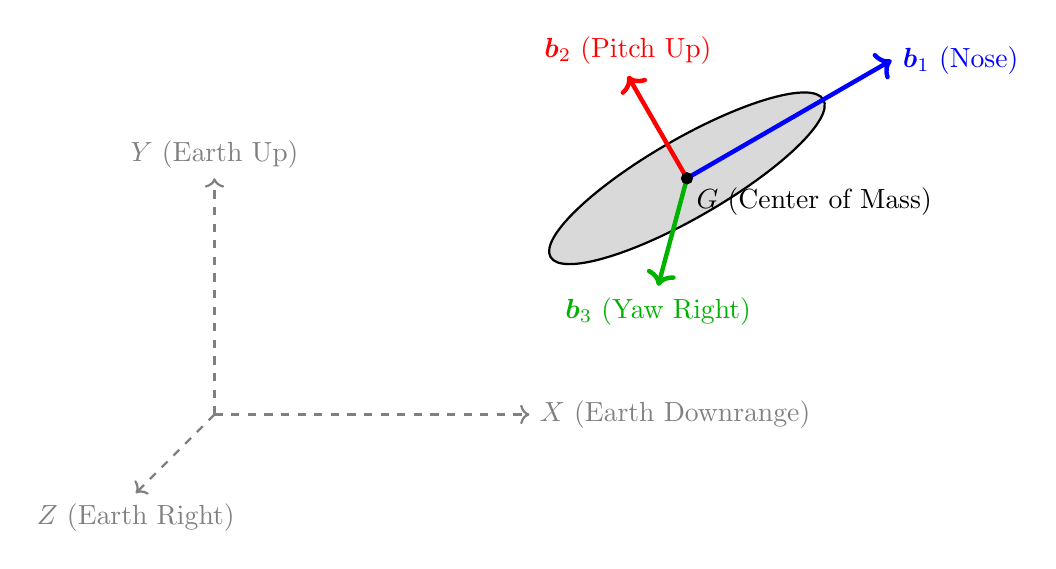
\begin{tikzpicture}
  % Inertial Frame
  \draw[->, thick, dashed, gray] (-2, -1) -- (-2, 2) node[above] {$Y$ (Earth Up)};
  \draw[->, thick, dashed, gray] (-2, -1) -- (2, -1) node[right] {$X$ (Earth Downrange)};
  \draw[->, thick, dashed, gray] (-2, -1) -- (-3, -2) node[below] {$Z$ (Earth Right)};
  
  % Bullet
  \draw[fill=gray!30, thick, rotate around={30:(4,2)}] (4,2) ellipse (2 and 0.5);
  
  % Body Frame
  \draw[->, ultra thick, blue, rotate around={30:(4,2)}] (4,2) -- (7, 2) node[right] {$\bm{b}_1$ (Nose)};
  \draw[->, ultra thick, red, rotate around={30:(4,2)}] (4,2) -- (4, 3.5) node[above] {$\bm{b}_2$ (Pitch Up)};
  \draw[->, ultra thick, green!70!black, rotate around={30:(4,2)}] (4,2) -- (3, 1) node[below] {$\bm{b}_3$ (Yaw Right)};
  
  % Center of mass
  \filldraw[black] (4,2) circle (2pt) node[below right] {$G$ (Center of Mass)};
\end{tikzpicture}
\caption{The Earth-fixed inertial frame versus the bullet's Body-fixed frame. As the bullet pitches and yaws, the body frame rotates independently of the earth frame.}
\label{fig:6dof_frames}
\end{figure}

\subsection{Euler Angles and Orientation}

The instantaneous orientation of the bullet's body frame relative to the stationary inertial frame is described by three Euler angles in the aerospace (yaw-pitch-roll) convention:

\begin{itemize}[nosep]
  \item $\psi$: yaw angle (rotation about $\bm{e}_y$)
  \item $\vartheta$: pitch angle (rotation about intermediate axis)
  \item $\varphi$: roll (spin) angle (rotation about $\bm{b}_1$)
\end{itemize}

The rotation matrix from inertial to body frame is:
\begin{equation}
  \bm{R} = \bm{R}_1(\varphi)\,\bm{R}_2(\vartheta)\,\bm{R}_3(\psi)
  \label{eq:rotation_matrix}
\end{equation}

\subsection{The 12-Component State Vector}

The full state vector is:
\begin{equation}
  \bm{Y} = \bigl(x,\; y,\; z,\; u,\; v,\; w,\; \varphi,\; \vartheta,\; \psi,\; p,\; q,\; r\bigr)^T
  \label{eq:6dof_state}
\end{equation}
where $(x,y,z)$ is position, $(u,v,w)$ is velocity in the inertial frame, $(\varphi, \vartheta, \psi)$ are Euler angles, and $(p, q, r)$ are angular velocity components in the body frame: $p$ is the spin rate about $\bm{b}_1$, and $q$, $r$ are pitch and yaw rates.

\section{Translational Equations of Motion}

Newton's second law in the inertial frame:
\begin{equation}
  \boxed{m\,\frac{\dd \vvec}{\dd t} = \bm{F}_{\mathrm{grav}} + \bm{F}_{\mathrm{drag}} + \bm{F}_{\mathrm{lift}} + \bm{F}_{\mathrm{Magnus}} + \bm{F}_{\mathrm{pitch\,damp}}}
  \label{eq:6dof_trans}
\end{equation}

\subsection{Total Angle of Attack}

The total angle of attack $\alpha_t$ is the angle between the velocity vector $\vvec$ and the body symmetry axis $\bm{b}_1$:
\begin{equation}
  \alpha_t = \arccos\left(\frac{\vvec \cdot \bm{b}_1}{\|\vvec\|}\right)
  \label{eq:total_aoa}
\end{equation}

For small angles, this decomposes into:
\begin{align}
  \alpha &\approx \vartheta - \gamma \quad \text{(pitch-plane angle of attack)} \\
  \beta  &\approx \psi_b - \psi_v \quad \text{(yaw-plane angle of attack)}
\end{align}
where $\gamma$ is the flight path angle.

\subsection{Aerodynamic Force Components}

All forces are expressed in terms of dimensionless coefficients, reference area $A = \pi d^2/4$, and dynamic pressure $\bar{q} = \frac{1}{2}\rho v^2$:

\textbf{Axial drag force} (opposing velocity along the symmetry axis):
\begin{equation}
  F_{\mathrm{drag}} = -\bar{q}\,A\,C_{D_0}(\Mach) - \bar{q}\,A\,C_{D_{\alpha^2}}(\Mach)\,\alpha_t^2
  \label{eq:6dof_drag}
\end{equation}
where $C_{D_0}$ is the zero-yaw drag coefficient and $C_{D_{\alpha^2}}$ is the yaw-drag coefficient.

\textbf{Normal (lift) force} (perpendicular to the symmetry axis, in the yaw plane):
\begin{equation}
  F_N = \bar{q}\,A\,C_{N_\alpha}(\Mach)\,\alpha_t
  \label{eq:6dof_lift}
\end{equation}
where $C_{N_\alpha}$ is the normal force derivative (lift-curve slope).

\textbf{Magnus force} (perpendicular to both the spin axis and the velocity--axis plane):
\begin{equation}
  F_{\mathrm{Magnus}} = \bar{q}\,A\,C_{N_{p\alpha}}(\Mach)\,\frac{p\,d}{2\,v}\,\alpha_t
  \label{eq:6dof_magnus_force}
\end{equation}

\section{Rotational Equations of Motion}

The general rotational equation for a rigid body in compact tensor form is:
\begin{equation}
  \boxed{\dot{\bm{\omega}} = \bm{I}^{-1}\!\left(\bm{M} - \bm{\omega} \times \bm{I}\,\bm{\omega}\right)}
  \label{eq:euler_tensor}
\end{equation}
where $\bm{I}$ is the inertia tensor, $\bm{\omega} = (p, q, r)^T$ is the angular velocity in the body frame, and $\bm{M}$ is the total external moment. The cross-product term $\bm{\omega} \times \bm{I}\,\bm{\omega}$ represents the gyroscopic coupling.

For an axially symmetric projectile (body of revolution) with $I_x$ (axial) and $I_y = I_z$ (transverse), the inertia tensor is diagonal and Eq.~\eqref{eq:euler_tensor} expands to the scalar Euler equations:

\begin{align}
  I_x\,\dot{p} &= M_x \label{eq:euler_p}\\
  I_y\,\dot{q} + (I_x - I_y)\,p\,r &= M_q \label{eq:euler_q}\\
  I_y\,\dot{r} - (I_x - I_y)\,p\,q &= M_r \label{eq:euler_r}
\end{align}

\subsection{Aerodynamic Moments}

\textbf{Overturning (pitching) moment} --- the moment that tends to increase the angle of attack:
\begin{equation}
  M_{\mathrm{pitch}} = \bar{q}\,A\,d\,C_{M_\alpha}(\Mach)\,\alpha_t
  \label{eq:overturning_moment}
\end{equation}
where $C_{M_\alpha}$ is the pitching moment coefficient derivative. For statically stable configurations, $C_{M_\alpha} < 0$ (restoring moment). For bullets, $C_{M_\alpha} > 0$ (statically unstable; stability comes from spin).

\textbf{Spin-damping moment} --- the torque that decelerates spin:
\begin{equation}
  M_{\mathrm{spin}} = \bar{q}\,A\,d^2\,C_{l_p}(\Mach)\,\frac{p\,d}{2\,v}
  \label{eq:spin_damping}
\end{equation}
where $C_{l_p} < 0$ is the spin-damping coefficient.

\textbf{Pitch-damping moment} --- opposes pitch/yaw rate:
\begin{equation}
  M_{\mathrm{damp}} = \bar{q}\,A\,d^2\,\left(C_{M_q} + C_{M_{\dot{\alpha}}}\right)\,\frac{d}{2\,v}\,(q \text{ or } r)
  \label{eq:pitch_damping}
\end{equation}

\textbf{Magnus moment}:
\begin{equation}
  M_{\mathrm{Magnus}} = \bar{q}\,A\,d^2\,C_{M_{p\alpha}}(\Mach)\,\frac{p\,d}{2\,v}\,\alpha_t
  \label{eq:magnus_moment}
\end{equation}

\subsection{Summary of Moment Components}

The total moments about each body axis:
\begin{align}
  M_x &= \bar{q}\,A\,d^2\,C_{l_p}\,\frac{p\,d}{2v} \label{eq:Mx}\\
  M_q &= \bar{q}\,A\,d\left[C_{M_\alpha}\,\alpha - C_{M_{p\alpha}}\,\frac{pd}{2v}\,\beta + (C_{M_q}+C_{M_{\dot{\alpha}}})\,\frac{qd}{2v}\right] \label{eq:Mq}\\
  M_r &= \bar{q}\,A\,d\left[C_{M_\alpha}\,\beta + C_{M_{p\alpha}}\,\frac{pd}{2v}\,\alpha + (C_{M_q}+C_{M_{\dot{\alpha}}})\,\frac{rd}{2v}\right] \label{eq:Mr}
\end{align}

\section{Kinematic Equations}

The Euler angle rates relate to the body-frame angular velocities:
\begin{align}
  \dot{\varphi} &= p + (q\sin\varphi + r\cos\varphi)\tan\vartheta \label{eq:kin_phi}\\
  \dot{\vartheta} &= q\cos\varphi - r\sin\varphi \label{eq:kin_theta}\\
  \dot{\psi} &= (q\sin\varphi + r\cos\varphi)\sec\vartheta \label{eq:kin_psi}
\end{align}

For small angles of attack ($\alpha_t < 10^{\circ}$), typical of rifle bullets, these simplify considerably.

\section{Quaternion Formulation (Singularity-Free)}

The Euler-angle formulation has a singularity at $\vartheta = \pm 90^{\circ}$ (gimbal lock). For robust numerical integration, the unit quaternion $\bm{q} = (q_0, q_1, q_2, q_3)^T$ is preferred:
\begin{equation}
  \frac{\dd}{\dd t}\begin{pmatrix}q_0\\q_1\\q_2\\q_3\end{pmatrix}
  = \frac{1}{2}\begin{pmatrix}
    0 & -p & -q & -r\\
    p &  0 &  r & -q\\
    q & -r &  0 &  p\\
    r &  q & -p &  0
  \end{pmatrix}
  \begin{pmatrix}q_0\\q_1\\q_2\\q_3\end{pmatrix}
  \label{eq:quat_ode}
\end{equation}

The rotation matrix from the quaternion:
\begin{equation}
  \bm{R} = \begin{pmatrix}
    1-2(q_2^2+q_3^2) & 2(q_1 q_2 - q_0 q_3) & 2(q_1 q_3 + q_0 q_2)\\
    2(q_1 q_2 + q_0 q_3) & 1-2(q_1^2+q_3^2) & 2(q_2 q_3 - q_0 q_1)\\
    2(q_1 q_3 - q_0 q_2) & 2(q_2 q_3 + q_0 q_1) & 1-2(q_1^2+q_2^2)
  \end{pmatrix}
  \label{eq:quat_to_R}
\end{equation}

After each integration step, renormalize: $\bm{q} \leftarrow \bm{q}/\|\bm{q}\|$.

\section{Aerodynamic Coefficient Database}

\subsection{Typical Values for Match Bullets}

The aerodynamic coefficients are functions of Mach number. Typical values for a 6.5\,mm, 140\,gr VLD match bullet at $\Mach \approx 2.4$ (muzzle) \citep{mccoy1999modern, carlucci2007ballistics}:

\begin{table}[H]
\centering
\caption{Typical aerodynamic coefficients for a 6.5\,mm 140\,gr VLD match bullet}
\label{tab:aero_coeffs}
\begin{tabular}{@{}lccl@{}}
\toprule
\textbf{Coefficient} & \textbf{Symbol} & \textbf{Typical Value} & \textbf{Description} \\
\midrule
Zero-yaw drag & $C_{D_0}$ & 0.15--0.30 & From G7 table via BC \\
Yaw drag & $C_{D_{\alpha^2}}$ & 2.0--5.0 & Drag increase with yaw \\
Lift-curve slope & $C_{N_\alpha}$ & 2.0--3.5 & Normal force per rad \\
Overturning moment & $C_{M_\alpha}$ & 2.0--4.0 & Destabilizing (positive) \\
Spin damping & $C_{l_p}$ & $-0.005$ to $-0.02$ & Retards spin \\
Pitch damping & $C_{M_q}+C_{M_{\dot\alpha}}$ & $-5$ to $-15$ & Damps yaw oscillation \\
Magnus force & $C_{N_{p\alpha}}$ & $-0.5$ to $+0.5$ & Cross-spin force \\
Magnus moment & $C_{M_{p\alpha}}$ & $-0.5$ to $+0.5$ & Cross-spin moment \\
\bottomrule
\end{tabular}
\end{table}

\default{Values in the Julia implementation when not user-specified.}

\subsection{Deriving $C_{D_0}$ from the Ballistic Coefficient}

The zero-yaw drag coefficient relates directly to the standard drag model and the ballistic coefficient:
\begin{equation}
  C_{D_0}(\Mach) = i \cdot C_D^{\mathrm{std}}(\Mach) = \frac{\sd}{\Bc}\,C_D^{\mathrm{std}}(\Mach)
  \label{eq:cd0_from_bc}
\end{equation}

This allows the 6-DOF model to use the same BC input as the 3-DOF model for the dominant drag term.

\section{Moments of Inertia}

For a rotationally symmetric bullet of mass $m$, length $L$, and diameter $d$:
\begin{align}
  I_x &\approx \frac{1}{2}\,m\,r_g^2 \quad \text{(axial, about symmetry axis)} \label{eq:Ix}\\
  I_y &= I_z \approx m\left(\frac{L^2}{12} + \frac{r_g^2}{4}\right) \quad \text{(transverse)} \label{eq:Iy}
\end{align}
where $r_g = d/2$ is the radius of gyration. For a typical match bullet, $I_y/I_x \approx 5$--$10$.

\section{Spin Rate and Initial Conditions}

The initial spin rate from the barrel twist rate $\tau$ (inches/turn):
\begin{equation}
  p_0 = \frac{2\pi\,v_0}{\tau}
  \label{eq:initial_spin}
\end{equation}

For a 1:8 twist barrel at 2700\,fps: $p_0 = 2\pi \times 2700/(8/12) = 2\pi \times 4050 \approx 25{,}447\;\text{rad/s}$ ($\approx 243{,}000\;\text{RPM}$).

\section{Stability Revisited from 6-DOF Theory}

\subsection{Gyroscopic Stability}

From the linearized 6-DOF equations, the gyroscopic stability factor is rigorously:
\begin{equation}
  S_g = \frac{I_x^2\,p^2}{2\,\rho\,A\,d\,I_y\,v^2\,C_{M_\alpha}}
  \label{eq:sg_6dof}
\end{equation}

This is the exact form from which the Miller approximation \eqref{eq:miller_sg} is derived.

\subsection{Dynamic Stability}

The dynamic stability factor from the 6-DOF linearization:
\begin{equation}
  S_d = \frac{2\,C_{N_\alpha}}{C_{M_\alpha}}\cdot\frac{1}{S_g(S_g-1)}\cdot\left(\frac{C_{N_\alpha} + \frac{2m}{\rho A d}\,k_t^2}{C_{M_q}+C_{M_{\dot{\alpha}}}}\right)^2
  \label{eq:sd_6dof}
\end{equation}

Full stability requires $S_g > 1$ and $0 < S_d < 2$.

\section{Comparison: 3-DOF vs.\ 6-DOF}

\begin{table}[H]
\centering
\caption{Comparison of 3-DOF and 6-DOF models}
\label{tab:3dof_vs_6dof}
\begin{tabularx}{\textwidth}{@{}lXX@{}}
\toprule
\textbf{Feature} & \textbf{3-DOF} & \textbf{6-DOF} \\
\midrule
State variables & 6 (position + velocity) & 13 (+ quaternion + angular velocity) \\
Spin drift & Empirical (Litz formula) & Predicted from first principles \\
Yaw/precession & Not modeled & Fully resolved \\
Magnus force & Neglected or lumped & Computed from $C_{N_{p\alpha}}$ \\
Transonic behavior & No yaw prediction & Predicts instability onset \\
Aerodynamic data & BC only & BC + 7 additional coefficients \\
Computation speed & $\sim$0.01\,s & $\sim$0.1--0.5\,s \\
Accuracy at 1000\,yd & $< 0.5\;\text{MOA}$ (with corrections) & $< 0.1\;\text{MOA}$ \\
\bottomrule
\end{tabularx}
\end{table}

For most competition shooting, the 3-DOF model with empirical spin drift and Coriolis corrections is sufficient. The 6-DOF model is valuable for: bullet design evaluation, predicting transonic stability limits, understanding anomalous dispersion, and academic study.

\section{Julia Implementation: 6-DOF Solver}

The 6-DOF solver is implemented in the \texttt{SixDOF} module within \texttt{CompetitionBallistics.jl} (Appendix~\ref{app:julia_file}). Key structures:

\begin{lstlisting}[caption={6-DOF solver usage example},label={lst:6dof_example}]
using .CompetitionBallistics.SixDOF

aero = AeroCoefficients6DOF(
    Cd0_func  = (Ma) -> cd_g7(Ma) * 1.02,  # from BC
    Cda2      = 3.5,       # yaw drag
    CNa       = 2.8,       # lift-curve slope
    CMa       = 3.2,       # overturning moment
    Clp       = -0.010,    # spin damping
    CMq_CMad  = -8.0,      # pitch damping sum
    CNpa      = 0.1,       # Magnus force
    CMpa      = -0.2,      # Magnus moment
)

params6 = ShotParameters6DOF(
    mass_grains=140.0, caliber_in=0.264,
    bullet_length_in=1.34,
    muzzle_vel_fps=2700.0, twist_in=8.0,
    initial_yaw_deg=0.5,  # typical muzzle yaw
    aero=aero,
)

traj = solve_6dof(params6)
\end{lstlisting}


% ============================================================================
\chapter{Angular Measurement and Sighting Systems}
\label{ch:sighting}

\section{Motivation: Speaking the Language of the Scope}

All the ballistic math in the world is useless if you cannot translate it into a physical adjustment on the rifle scope. A ballistic solver calculates the drop of a bullet in linear units (like inches or centimeters). However, rifle scopes do not adjust in linear units; they adjust by changing angles. 

When you turn the elevation dial on a scope, you are physically tilting the optic downward relative to the barrel so that you are forced to aim the barrel upward to compensate for drop. To hit the target, we must convert linear distance at the target ($\Delta y$) into an angular measurement at the scope. The two dominant angular languages in shooting are Minute of Angle (MOA) and Milliradian (Mil).

\section{Minute of Angle (MOA)}

A circle has 360 degrees. A Minute of Angle is exactly $1/60^{\text{th}}$ of one degree.

First, let's verify what this small angle actually means in radians:
\begin{equation}
  1\;\text{MOA} = \frac{1^{\circ}}{60} \times \frac{\pi}{180^{\circ}} = \SI{2.9089e-4}{\radian}
  \label{eq:moa_rad}
\end{equation}

Because tangent of a very small angle is approximately equal to the angle in radians ($\tan(\theta) \approx \theta$), we can calculate exactly how much physical distance 1 MOA covers at 100 yards ($R = 3600$ inches):
$$ \Delta y = R \cdot \theta_{\text{rad}} = 3600 \cdot \SI{2.9089e-4}{} \approx 1.047 \text{ inches} $$

This is where the common (but slightly inaccurate) shooter's approximation comes from: $1\;\text{MOA} \approx 1$ inch at \SI{100}{\yard}. 

To convert your calculated bullet drop ($\Delta y$) at range $R$ (ensuring both are in the same linear units, e.g., inches) into a scope dial adjustment in MOA, use this exact formula:
\begin{equation}
  \boxed{\text{MOA Dial Adjustment} = \frac{\Delta y}{R} \cdot \frac{180 \times 60}{\pi} \approx \frac{\Delta y}{R} \cdot 3437.75}
  \label{eq:moa_calc}
\end{equation}

\section{Milliradian (Mil, MRAD)}

While MOA is mathematically tied to the 360-degree circle (popular in the US), the Milliradian system operates on pure base-10 metric logic (popular internationally and in military applications). A radian is the angle subtended when the arc length equals the radius. A milliradian is $1/1000^{\text{th}}$ of a radian.

\begin{equation}
  1\;\text{mil} = \SI{0.001}{\radian} 
  \label{eq:mil}
\end{equation}

Because $1 \text{ mil} = 0.001 \text{ rad}$, the math is incredibly elegant: 1 mil is exactly 1 meter at 1,000 meters, 10 centimeters at 100 meters, or $3.6$ inches at 100 yards.

For mixed scope usage, the hard conversion is: $1\;\text{mil} = 3.438\;\text{MOA}$.

To calculate the necessary dial adjustment on a Mil-based scope, using drop $\Delta y$ and range $R$ (again, matching linear units):
\begin{equation}
  \boxed{\text{Mil Dial Adjustment} = \frac{\Delta y}{R} \times 1000}
  \label{eq:mil_calc}
\end{equation}


% ============================================================================
\chapter{Reloading Guide for Competition Shooters}
\label{ch:reloading}

\section{Motivation: Controlling the Variables}

No amount of ballistic solver software can make up for inconsistent ammunition. Factory ammunition, even "match grade," is mass-produced and subject to tolerance stacking. To guarantee extreme precision (Standard Deviations in velocity below 10 FPS), competition shooters handload their own ammunition. Reloading is fundamentally about controlling variables—neck tension, seating depth, powder charge, and concentricity—so that every single round possesses the exact same interior ballistics.

\textbf{Safety Warning:} Handloading deals with immense explosive pressures near your face. Always cross-reference with current published load data from powder manufacturers. Start 10\% below listed maximum charges and work up carefully while watching for pressure signs on the brass primer.

\section{Cartridge Selection for Competition}

\begin{table}[H]
\centering
\caption{Popular competition cartridges and their characteristics}
\label{tab:cartridges}
\small
\begin{tabularx}{\textwidth}{@{}lccccX@{}}
\toprule
\textbf{Cartridge} & \textbf{Bullet (gr)} & \textbf{$v_0$ (fps)} & \textbf{BC (G7)} & \textbf{Barrel} & \textbf{Discipline} \\
\midrule
6mm BR & 105--108 & 2850--2950 & .225--.275 & 26--28 & Benchrest, F-Class \\
6mm Creedmoor & 105--115 & 2950--3100 & .255--.290 & 26--28 & PRS, NRL, F-Class \\
6mm Dasher & 105--115 & 2950--3050 & .225--.290 & 26--28 & PRS, NRL \\
6.5 Creedmoor & 130--147 & 2550--2800 & .255--.340 & 24--26 & PRS, NRL, F-Class \\
6.5$\times$47 Lapua & 130--147 & 2650--2850 & .255--.340 & 26--28 & Palma variant \\
.284 Win & 180 & 2850--2950 & .340--.365 & 28--30 & F-Class Open \\
.308 Win & 155--185 & 2550--2800 & .220--.275 & 24--30 & Palma, Tactical \\
.223 Rem & 69--80 & 2700--3000 & .145--.200 & 20--26 & Service Rifle \\
.300 Win Mag & 190--230 & 2800--3000 & .310--.415 & 26--30 & F-Class Open \\
.338 Lapua Mag & 250--300 & 2700--2900 & .370--.450 & 27--30 & ELR \\
\bottomrule
\end{tabularx}
\end{table}

\section{Propellant Selection}

Selecting the proper propellant is a balance between achieving the desired muzzle velocity ($v_0$), maintaining a low velocity spread ($\sigma_v$), and ensuring safety across a wide range of temperatures. Propellants are broadly categorized into single-base (nitrocellulose-only) and double-base (nitrocellulose and nitroglycerine). Single-base propellants generally offer cleaner burning and superior temperature stability, whereas double-base propellants provide higher energy density (resulting in higher velocities) at the expense of higher thermal sensitivity and increased barrel throat erosion. Table~\ref{tab:propellants} summarizes popular propellants used in competition shooting, highlighting their burn rate and relative temperature stability.

\begin{table}[H]
\centering
\caption{Popular propellants for competition rifle cartridges}
\label{tab:propellants}
\small
\begin{tabularx}{\textwidth}{@{}llcX@{}}
\toprule
\textbf{Propellant} & \textbf{Burn Rate} & \textbf{Temp Stable?} & \textbf{Typical Cartridges} \\
\midrule
Hodgdon Varget & Medium & Yes (Extreme) & .308, .223, 6.5 CM, 6BR \\
Hodgdon H4350 & Med-slow & Yes (Extreme) & 6.5 CM, 6 CM, .284, .260 \\
Hodgdon H4895 & Medium & Yes (Extreme) & 6BR, .308, .223 \\
Alliant RL-16 & Med-slow & Yes (ETS) & 6.5 CM, 6 CM, 6mm BR \\
Vihtavuori N140 & Medium & Moderate & 6mm BR, .308, .223 \\
Vihtavuori N150 & Med-slow & Moderate & 6.5 CM, 6 CM, .260 \\
Vihtavuori N555 & Medium & Yes & 6mm BR, 6 Dasher \\
Vihtavuori N565 & Med-slow & Yes & 6.5 CM, 6 CM, 6.5$\times$47 \\
IMR 4451 & Med-slow & Yes (Enduron) & 6.5 CM, 6 CM, .308 \\
Reload Swiss RS52 & Medium & Moderate & .308 Win, 6mm BR, 6.5 CM \\
Reload Swiss RS60 & Med-slow & No (Impregnated) & 6.5 CM, .260, 6.5$\times$55 \\
Vectan Tubal 5000 & Medium & No & .308 Win, .30-30, 8$\times$57 \\
\bottomrule
\end{tabularx}
\end{table}

\section{Representative Load Data}

\textbf{Disclaimer:} Reference only. Always consult current manufacturer manuals. Start 10\% below maximum.

\begin{table}[H]
\centering
\caption{6.5 Creedmoor representative loads (24-inch barrel)}
\label{tab:65cm_loads}
\begin{tabular}{@{}llcccc@{}}
\toprule
\textbf{Bullet} & \textbf{Propellant} & \textbf{Charge (gr)} & \textbf{COAL (in)} & \textbf{$v_0$ (fps)} & \textbf{Press.} \\
\midrule
140 Berger Hybrid & H4350 & 40.0--42.5 & 2.800 & 2650--2760 & Near max \\
147 Hornady ELD-M & H4350 & 38.5--41.0 & 2.830 & 2550--2660 & Near max \\
130 Berger Hybrid & H4350 & 41.0--43.5 & 2.810 & 2750--2880 & Near max \\
140 Sierra MK & RL-16 & 39.0--41.5 & 2.800 & 2640--2750 & Near max \\
147 Hornady ELD-M & N565 & 39.5--42.0 & 2.830 & 2570--2680 & Near max \\
\bottomrule
\end{tabular}
\end{table}

\begin{table}[H]
\centering
\caption{.308 Winchester representative loads (24-inch barrel)}
\label{tab:308_loads}
\begin{tabular}{@{}llcccc@{}}
\toprule
\textbf{Bullet} & \textbf{Propellant} & \textbf{Charge (gr)} & \textbf{COAL (in)} & \textbf{$v_0$ (fps)} & \textbf{Press.} \\
\midrule
175 Sierra MK & Varget & 42.0--44.5 & 2.800 & 2550--2680 & Near max \\
155 Berger Hybrid & Varget & 44.5--47.0 & 2.800 & 2750--2870 & Near max \\
168 Sierra MK & Varget & 43.0--45.5 & 2.800 & 2600--2720 & Near max \\
175 Sierra MK & N150 & 43.0--45.0 & 2.800 & 2570--2670 & Near max \\
\bottomrule
\end{tabular}
\end{table}

\begin{table}[H]
\centering
\caption{6mm Creedmoor representative loads (26-inch barrel)}
\label{tab:6cm_loads}
\begin{tabular}{@{}llcccc@{}}
\toprule
\textbf{Bullet} & \textbf{Propellant} & \textbf{Charge (gr)} & \textbf{COAL (in)} & \textbf{$v_0$ (fps)} & \textbf{Press.} \\
\midrule
105 Berger Hybrid & H4350 & 39.5--42.0 & 2.800 & 3000--3100 & Near max \\
108 Berger BT Tgt & H4350 & 39.0--41.5 & 2.800 & 2950--3070 & Near max \\
115 Berger Hybrid & RL-16 & 38.0--40.5 & 2.810 & 2880--2990 & Near max \\
105 Hornady ELD-M & N565 & 38.5--41.0 & 2.790 & 2980--3080 & Near max \\
109 Berger LRHT & H4350 & 38.5--41.0 & 2.810 & 2950--3060 & Near max \\
\bottomrule
\end{tabular}
\end{table}

\begin{table}[H]
\centering
\caption{6mm BR Norma representative loads (26-inch barrel)}
\label{tab:6br_loads}
\begin{tabular}{@{}llcccc@{}}
\toprule
\textbf{Bullet} & \textbf{Propellant} & \textbf{Charge (gr)} & \textbf{COAL (in)} & \textbf{$v_0$ (fps)} & \textbf{Press.} \\
\midrule
105 Berger Hybrid & Varget & 29.0--30.5 & 2.350 & 2850--2950 & Near max \\
105 Berger Hybrid & N140 & 29.5--31.0 & 2.350 & 2870--2960 & Near max \\
108 Berger BT Tgt & Varget & 28.5--30.0 & 2.350 & 2820--2920 & Near max \\
108 Berger BT Tgt & N555 & 29.0--30.5 & 2.350 & 2850--2950 & Near max \\
105 Lapua Scenar & H4895 & 28.5--30.0 & 2.340 & 2830--2930 & Near max \\
107 Sierra MK & Varget & 28.5--30.0 & 2.350 & 2830--2930 & Near max \\
\bottomrule
\end{tabular}
\end{table}

% ============================================================================
\section{Complete Worked Example: 6mm BR at 1000 Yards}
\label{sec:6br_example}

This section walks through a complete ballistic simulation for a 6mm BR Norma benchrest/F-Class load, from component data through atmospheric correction to a full trajectory table with all secondary effects. This serves as a template for any cartridge.

\subsection{Step 1: Component Data}

Our load:
\begin{itemize}[nosep]
  \item \textbf{Bullet:} Berger 105\,gr Hybrid Target, 6mm (.243 cal)
  \item \textbf{BC (G7):} 0.275 \citep{litz2015ballistic}
  \item \textbf{Bullet length:} 1.292 in.\ (manufacturer specification)
  \item \textbf{Propellant:} Vihtavuori N140, 30.2\,gr
  \item \textbf{Muzzle velocity:} 2920\,fps (from 26-inch barrel, verified by chronograph)
  \item \textbf{Barrel twist:} 1:7.5 right-hand
  \item \textbf{Brass:} Lapua 6mm BR, weight-sorted $\pm$0.5\,gr
  \item \textbf{Primer:} CCI BR-4 small rifle benchrest
\end{itemize}

\subsection{Step 2: Stability Check}

Using the Miller formula \eqref{eq:miller_sg}:
\begin{align*}
  d &= 0.243\;\text{in.}, \quad l = 1.292/0.243 = 5.317\;\text{cal}, \quad T_w = 7.5/0.243 = 30.86\;\text{cal/turn} \\
  S_g &= \frac{30 \times 105}{30.86^2 \times 0.243^3 \times 5.317 \times (1 + 5.317^2)} \times \left(\frac{2920}{2800}\right)^{1/3} \times \frac{518.67}{518.67} \\
  &= \frac{3150}{30.86^2 \times 0.01435 \times 5.317 \times 29.27} \times 1.014 \\
  &\approx 1.50
\end{align*}

$S_g = 1.50 > 1.3$: well stabilized, and right at the threshold above which the bullet realises its full BC. The bullet will maintain gyroscopic stability down to approximately Mach 1.2 (about 1350\,fps), which occurs near 1100 yards for this load.

\subsection{Step 3: Atmospheric Conditions}

Match day conditions (summer F-Class match in Ottawa, Canada):
\begin{align*}
  T &= \SI{27.8}{\celsius} = 82\,\degF = 300.9\;\text{K} \\
  P &= 29.75\;\text{in Hg} = 100\,750\;\text{Pa} \\
  H &= 55\%, \quad \text{Altitude} = 250\;\text{ft}
\end{align*}

Air density from Eq.~\eqref{eq:rho_humid}:
\begin{align*}
  e_s &= 610.78 \times 10^{7.5 \times 27.7 / (27.7 + 237.3)} = 3695\;\text{Pa} \\
  e &= 0.55 \times 3695 = 2032\;\text{Pa} \\
  \rho &= \frac{100\,750 - 0.3783 \times 2032}{287.058 \times 300.9} = \frac{99\,981}{86\,380} = 1.1575\;\text{kg/m}^3
\end{align*}

Density ratio: $\rho/\rho_0 = 1.1575/1.2250 = 0.9449$. The air is 5.5\% less dense than standard, so the bullet will retain velocity longer and shoot approximately 0.8 MOA flatter at 1000 yards compared to standard conditions.

Speed of sound (at \SI{27.8}{\celsius}): $a = 20.047\sqrt{300.9} = 347.7\;\text{m/s}$.

Muzzle Mach number: $\Mach_0 = 890.0/347.7 = 2.56$ (well into the supersonic regime).

\subsection{Step 4: Solver Setup and Trajectory}

The complete Julia solver call for this scenario:

\begin{lstlisting}[caption={6mm BR complete trajectory example},label={lst:6br_example}]
params_6br = ShotParameters(
    # Bullet: Berger 105 Hybrid Target
    mass_grains     = 105.0,
    caliber_in      = 0.243,
    bc              = 0.275,        # G7
    drag_model      = :G7,

    # Launch
    muzzle_vel_fps  = 2920.0,
    sight_height_in = 1.5,
    zero_range_yd   = 100.0,

    # Atmosphere: Ottawa, summer match
    temp_F          = 82.0,         # 27.8 C
    pressure_inhg   = 29.75,
    humidity_pct    = 55.0,
    altitude_ft     = 250.0,

    # Wind: 8 mph from 2 o'clock (60 deg off nose)
    wind_speed_mph  = 8.0,
    wind_angle_deg  = 60.0,

    # Target
    target_range_yd = 1000.0,

    # Spin: 1:7.5 RH twist
    twist_in        = 7.5,
    twist_direction = 1,
    bullet_length_in = 1.10,

    # Location: Ottawa, ON
    latitude_deg    = 45.4,
    azimuth_deg     = 270.0,       # firing West
    enable_coriolis = true,
    enable_spin_drift = true,
)

trajectory_table(params_6br, step_yd=100)
\end{lstlisting}

The solver output for this configuration:

\begin{table}[H]
\centering
\caption{Computed trajectory: 6mm BR, 105 gr Berger Hybrid, $v_0 = 2920$ fps, \protect\SI{27.8}{\celsius} (82\protect\degF), 29.75 in Hg, 55\% RH. 8 mph wind at $60^{\circ}$. 100 yd zero. 1:7.5 RH twist, $45.4^{\circ}$N, firing West.}
\label{tab:6br_trajectory}
\small
\begin{tabular}{@{}rrrrrrrrr@{}}
\toprule
\textbf{Range} & \textbf{Drop} & \textbf{Elev} & \textbf{Vel} & \textbf{Mach} & \textbf{Energy} & \textbf{ToF} & \textbf{Wind} & \textbf{Spin} \\
\textbf{(yd)} & \textbf{(in)} & \textbf{(MOA)} & \textbf{(fps)} & & \textbf{(ft-lb)} & \textbf{(s)} & \textbf{(in)} & \textbf{(in)} \\
\midrule
100  &    0.0 &   0.0 & 2766 & 2.43 & 1784 & 0.106 &   0.3 & 0.0 \\
200  &  $-$2.3 &   1.1 & 2617 & 2.30 & 1597 & 0.219 &   1.5 & 0.1 \\
300  &  $-$9.0 &   2.9 & 2473 & 2.17 & 1427 & 0.339 &   3.6 & 0.2 \\
400  & $-$20.7 &   5.0 & 2334 & 2.05 & 1271 & 0.466 &   6.8 & 0.4 \\
500  & $-$38.2 &   7.3 & 2200 & 1.93 & 1129 & 0.602 &  11.1 & 0.7 \\
600  & $-$62.5 &  10.0 & 2070 & 1.82 & 1000 & 0.747 &  16.8 & 1.1 \\
700  & $-$94.8 &  12.9 & 1945 & 1.71 &  883 & 0.903 &  24.0 & 1.6 \\
800  &$-$136.5 &  16.3 & 1824 & 1.60 &  776 & 1.070 &  32.9 & 2.3 \\
900  &$-$189.5 &  20.1 & 1708 & 1.50 &  681 & 1.250 &  43.9 & 3.1 \\
1000 &$-$256.0 &  24.5 & 1596 & 1.40 &  594 & 1.445 &  57.0 & 4.1 \\
\bottomrule
\end{tabular}
\end{table}

\subsection{Step 5: Analysis of Results}

\textbf{Velocity retention.} The bullet arrives at 1000 yards at 1596 fps (Mach 1.40), still well above the transonic threshold ($\approx$1340 fps). The 6mm BR with a high-BC 105\,gr bullet retains adequate supersonic margin.

\textbf{Total elevation.} From the 100-yard zero, the shooter dials 24.5 MOA of elevation (approximately 7.1 mils). This is competitive with the 6.5 Creedmoor (28.5 MOA for 140 gr, Table~\ref{tab:drop_65cm}) despite the lighter bullet, thanks to the higher muzzle velocity.

\textbf{Wind deflection.} The 8 mph wind at $60^{\circ}$ produces a crosswind component $W_{\mathrm{cross}} = 8 \sin 60^{\circ} = 6.93$ mph and a headwind component $W_{\mathrm{head}} = 8 \cos 60^{\circ} = 4.0$ mph. The total wind deflection at 1000 yards is 57.0 inches (5.4 MOA). For a full-value 10 mph crosswind, this would scale to approximately 74 inches --- about 4\% more than the 6.5 Creedmoor (77.1 in.) but comparable, illustrating that the 6mm BR's higher velocity partly compensates for the lower BC.

\textbf{Spin drift.} The 1:7.5 RH twist produces 4.1 inches of rightward drift at 1000 yards (0.39 MOA). This is a systematic bias that should be dialed into the scope or included in the wind hold.

\textbf{Coriolis and E\"otv\"os.} Firing West at $45.4^{\circ}$N latitude:
\begin{itemize}[nosep]
  \item Horizontal Coriolis: $\approx 2.7$ inches right (0.26 MOA), same direction as spin drift.
  \item E\"otv\"os (firing West): $\approx 3.4$ inches \emph{down} (the bullet loses the ``boost'' of the Earth's rotation), adding about 0.3 MOA to the required elevation.
\end{itemize}

\textbf{Total horizontal correction:} Wind 57.0 in.\ $+$ spin drift 4.1 in.\ $+$ Coriolis 2.7 in.\ $= 63.8$ inches total rightward deflection (6.1 MOA).

\subsection{Step 6: Chronograph Validation}

A 20-round chronograph string from this load:
\begin{center}
\small
2918, 2925, 2914, 2928, 2920, 2916, 2922, 2919, 2927, 2921, \\
2915, 2923, 2926, 2917, 2920, 2924, 2919, 2922, 2916, 2925
\end{center}

Statistics: $\bar{v} = 2920.9$ fps, ES $= 14$ fps, SD $= 3.9$ fps. The SD of 3.9 fps produces a vertical dispersion of:
\begin{equation*}
  \sigma_y(1000\;\text{yd}) \approx 0.23 \times 3.9 = 0.90\;\text{inches} \quad (0.09\;\text{MOA})
\end{equation*}

This is well below the F-Class X-ring diameter (2.5 inches) and represents a benchrest-grade load.

\subsection{Step 7: DOPE Card Summary}

\begin{table}[H]
\centering
\caption{DOPE card: 6mm BR 105 Berger / N140 / 2920 fps. Ottawa, \protect\SI{27.8}{\celsius} (82\protect\degF), 29.75 inHg. Wind hold is per 1 mph full crosswind.}
\label{tab:6br_dope}
\begin{tabular}{@{}rccc@{}}
\toprule
\textbf{Range (yd)} & \textbf{Elevation (MOA)} & \textbf{Wind/1 mph (MOA)} & \textbf{Spin+Cor (MOA)} \\
\midrule
200 &  1.1 & 0.07 & 0.01 \\
300 &  2.9 & 0.11 & 0.03 \\
400 &  5.0 & 0.16 & 0.05 \\
500 &  7.3 & 0.21 & 0.08 \\
600 & 10.0 & 0.27 & 0.12 \\
700 & 12.9 & 0.33 & 0.17 \\
800 & 16.3 & 0.39 & 0.23 \\
900 & 20.1 & 0.47 & 0.30 \\
1000 & 24.5 & 0.54 & 0.39 \\
\bottomrule
\end{tabular}
\end{table}

This DOPE card gives the shooter all the information needed: dial the elevation, hold or dial the wind column multiplied by the estimated crosswind speed, and add the spin+Coriolis correction. The total process---from the mathematical models of Chapters 2--6 through the Julia solver of Chapter 7 to this practical output---represents the complete ballistic pipeline that this manual describes.

\section{Interpreting Chronograph Data}

\begin{align}
  \bar{v} &= \frac{1}{N}\sum_{i=1}^N v_i, \qquad
  \text{ES} = v_{\max} - v_{\min}, \qquad
  \text{SD} = \sqrt{\frac{1}{N-1}\sum_{i=1}^N (v_i - \bar{v})^2}
\end{align}

Target values: ES $< 20\;\text{fps}$ (excellent: $< 10$), SD $< 8\;\text{fps}$ (excellent: $< 4$).

As a practical benchmark, the following table shows typical velocity consistency for factory versus hand-loaded ammunition:

\begin{table}[H]
\centering
\caption{Typical velocity consistency: factory ammunition vs.\ optimized handloads}
\label{tab:velocity_consistency}
\small
\begin{tabular}{@{}lcc@{}}
\toprule
\textbf{Ammunition type} & \textbf{ES (m/s)} & \textbf{ES (fps)} \\
\midrule
Standard factory match    & 9--10  & 30--33 \\
Premium factory match     & 5--7   & 16--23 \\
Optimized handloads       & 2--3   & 7--10 \\
Benchrest-grade handloads & $<$2   & $<$7 \\
\bottomrule
\end{tabular}
\end{table}

The gap between factory and hand-loaded ammunition is the primary motivation for reloading in competition shooting: reducing velocity spread by a factor of 3--5 translates directly into tighter vertical dispersion at long range (see below).

\subsection{Velocity SD Impact on Vertical Dispersion}

\begin{equation}
  \sigma_y(R) \approx \left|\frac{\partial y}{\partial v_0}\right|_{R} \cdot \sigma_v
  \label{eq:vertical_sd}
\end{equation}


% ============================================================================
\chapter{Ballistic Reference Tables}
\label{ch:tables}

\section{Bullet Data for Common Competition Bullets}

\begin{table}[H]
\centering
\caption{Ballistic data for popular competition bullets \citep{litz2011applied, litz2015ballistic}}
\label{tab:bullet_data}
\small
\begin{tabular}{@{}lcccccc@{}}
\toprule
\textbf{Bullet} & \textbf{Wt (gr)} & \textbf{Cal} & \textbf{BC G1} & \textbf{BC G7} & \textbf{SD} & \textbf{Twist} \\
\midrule
Berger 105 Hyb 6mm & 105 & .243 & 0.536 & 0.275 & 0.254 & 1:7.5 \\
Berger 140 Hyb 6.5 & 140 & .264 & 0.607 & 0.311 & 0.287 & 1:8 \\
Hornady 147 ELD-M & 147 & .264 & 0.697 & 0.351 & 0.301 & 1:7.5 \\
Berger 180 Hyb 7mm & 180 & .284 & 0.683 & 0.350 & 0.319 & 1:8.5 \\
Sierra 175 MK .308 & 175 & .308 & 0.505 & 0.259 & 0.264 & 1:10 \\
Berger 185 Jugg .308 & 185 & .308 & 0.552 & 0.283 & 0.279 & 1:10 \\
Hornady 178 ELD-M & 178 & .308 & 0.535 & 0.274 & 0.268 & 1:10 \\
Berger 300 Hyb .338 & 300 & .338 & 0.818 & 0.419 & 0.375 & 1:9.4 \\
\bottomrule
\end{tabular}
\end{table}

\section{Sample Trajectory Table}

\begin{table}[H]
\centering
\caption{Trajectory: 6.5 CM, 140 gr Berger Hybrid, BC$_{\text{G7}}$ = 0.311, $v_0$ = 2700 fps, 100 yd zero, sea level standard atmosphere}
\label{tab:drop_65cm}
\small
\begin{tabular}{@{}rrrrrrrr@{}}
\toprule
\textbf{Range} & \textbf{Drop} & \textbf{Come-Up} & \textbf{Velocity} & \textbf{Energy} & \textbf{ToF} & \textbf{10 mph Wind} & \textbf{Spin Drift} \\
\textbf{(yd)} & \textbf{(in)} & \textbf{(MOA)} & \textbf{(fps)} & \textbf{(ft-lb)} & \textbf{(s)} & \textbf{(in)} & \textbf{(in)} \\
\midrule
100 & 0.0 & 0.0 & 2545 & 2015 & 0.115 & 0.5 & 0.0 \\
200 & $-$2.8 & 1.3 & 2396 & 1786 & 0.237 & 2.1 & 0.1 \\
300 & $-$10.7 & 3.4 & 2252 & 1578 & 0.365 & 5.0 & 0.3 \\
400 & $-$24.5 & 5.9 & 2113 & 1389 & 0.501 & 9.2 & 0.5 \\
500 & $-$45.0 & 8.6 & 1979 & 1219 & 0.646 & 15.1 & 0.9 \\
600 & $-$73.4 & 11.7 & 1851 & 1066 & 0.800 & 22.8 & 1.4 \\
700 & $-$111.0 & 15.1 & 1728 & 929 & 0.965 & 32.5 & 2.0 \\
800 & $-$159.5 & 19.0 & 1610 & 807 & 1.143 & 44.6 & 2.8 \\
900 & $-$221.1 & 23.5 & 1498 & 698 & 1.334 & 59.3 & 3.8 \\
1000 & $-$298.0 & 28.5 & 1393 & 604 & 1.541 & 77.1 & 5.1 \\
\bottomrule
\end{tabular}
\end{table}


% ============================================================================
\chapter{Special Topics}
\label{ch:special}

\section{Motivation: The Edges of the Envelope}

Standard exterior ballistics hold true while the bullet is flying supersonic. However, new bizarre aerodynamic phenomena occur when the bullet slows down and breaks the sound barrier in reverse (the transonic zone). This chapter briefly introduces edge-case ballistics that ruin otherwise perfect shots at extreme long ranges.

\section{Transonic Stability}

The dynamic stability factor $S_d$ must be considered alongside the gyroscopic stability factor $S_g$ \citep{mccoy1999modern}. For full stability: $S_g > 1.0$ and $0 < S_d < 2$.

As a bullet decelerates through the transonic zone ($0.9 \lesssim \Mach \lesssim 1.2$), the centre of pressure shifts rapidly and the aerodynamic damping can change sign, potentially causing a well-stabilized supersonic bullet to become dynamically unstable. The practical consequence is increased dispersion---often dramatically so---once the bullet enters this regime. Long-range competitors should therefore know at what range their chosen load crosses into the transonic zone and treat that as the effective maximum range for precision fire.

\begin{table}[H]
\centering
\caption{Approximate transonic transition ranges for common competition cartridges at sea-level standard conditions. The transonic zone is defined as $0.9 \leq \Mach \leq 1.1$ ($\approx\SI{310}{}$--$\SI{380}{\meter\per\second}$).}
\label{tab:transonic_ranges}
\small
\begin{tabular}{@{}llccc@{}}
\toprule
\textbf{Cartridge} & \textbf{Bullet (gr)} & \textbf{$v_0$ (m/s)} & \textbf{Enters transonic (m)} & \textbf{Subsonic (m)} \\
\midrule
.223 Rem        & 77 SMK          & 838  & $\approx$600  & $\approx$750 \\
.308 Win        & 155 Lapua Scenar & 860 & $\approx$750  & $\approx$950 \\
.308 Win        & 175 SMK         & 775  & $\approx$820  & $\approx$1075 \\
6.5 Creedmoor   & 140 Berger Hybrid & 823 & $\approx$950 & $\approx$1200 \\
.300 Win Mag    & 185 Berger Jugg  & 943  & $\approx$1275 & $\approx$1600 \\
.338 Lapua Mag  & 300 Berger Hybrid & 838 & $\approx$1500 & $\approx$1900 \\
\bottomrule
\end{tabular}
\end{table}

Bullets with higher BC values and higher muzzle velocities remain supersonic longer, but the relationship is not linear: the steep drag rise in the transonic zone means that once a bullet begins to slow through $\Mach \approx 1.1$, it decelerates rapidly. The solver in Chapter~\ref{ch:solver} captures this behavior through the fine resolution of the G7 drag table in the transonic region.

\section{Inclined Fire (Rifleman's Rule)}

\begin{equation}
  R_{\mathrm{effective}} = R_{\mathrm{slant}} \cdot \cos\alpha
  \label{eq:riflemans_rule}
\end{equation}

The perpendicular gravity component $g_{\perp} = g\cos\alpha$ causes the bullet to drop away from the line of sight. Since $\cos\alpha < 1$ for any nonzero inclination (up or down), the drop is always less than flat fire.

Rather than applying the approximate range-scaling of Eq.~\eqref{eq:riflemans_rule}
as a post-correction, the solver handles inclination exactly: it resolves gravity
in the line-of-sight frame, applying $g_{\perp} = g\cos\alpha$ perpendicular to the
sight line and $g_{\parallel} = g\sin\alpha$ along the flight path, then integrates
normally. This captures the slight up/down asymmetry (the along-path component
accelerates a descending shot and decelerates a climbing one) that the pure
cosine rule omits. For the reference 6.5\,mm load at $\pm 30^{\circ}$ and
\SI{1000}{\yard}, the drop along the sight line falls from $-300.6$ inches (flat) to
$-258.4$ inches (uphill) and $-252.2$ inches (downhill).

These three figures were $-272$, $-233$ and $-228$ until 2026-08-14 --- about
10\,\% shallower, in a constant ratio. They predate the reference-area correction
on $\Cd$ (the BRL tables refer drag to $\pi d^2/4$, so the solver carries a factor
$4/\pi$; omitting it understates drag by 27\,\%). Both implementations now return
the values above, to the digit.

\section{Barrel Harmonics and Optimal Charge Weight}

Barrel vibrations cause the muzzle to describe an elliptical pattern at the moment of bullet exit. The OCW method seeks charge weights where the muzzle vertical angle is at an extremum, creating a flat spot that compensates for velocity variation.


% ============================================================================
\chapter{Error Budget and Sensitivity Analysis}
\label{ch:sensitivity}

\section{Motivation: Knowing Your Weakest Link}

In competition shooting, you are constantly fighting physics. An "Error Budget" is a mathematical tool to figure out which physical variable is most likely to cause you to miss. It helps a shooter answer the question: \emph{"Should I spend \$500 on a better laser rangefinder, or \$500 on a better scale to weigh my gun powder?"}

By running a sensitivity analysis, we systematically slightly tweak one variable at a time (like making the wind \SI{1}{\mph} faster, or the muzzle velocity \SI{10}{\fps} slower) and observe how much the bullet's impact point moves at a specific range.

\section{Sensitivity Coefficients}

For any given trajectory output $Y$ (such as vertical drop or wind deflection) at a specific range $R$, we can define the sensitivity $S_i$ to a specific parameter $p_i$:

Let's define the terms:
\begin{itemize}[noitemsep]
    \item $Y$: The output of the ballistic solver (e.g., vertical drop in inches).
    \item $p_i$: The input parameter being analyzed (e.g., Muzzle Velocity in fps).
    \item $\Delta p_i$: A small, realistic uncertainty or error in that parameter.
\end{itemize}

\begin{equation}
  S_i = \frac{\partial Y}{\partial p_i} \approx \frac{Y(p_i + \Delta p_i) - Y(p_i - \Delta p_i)}{2\,\Delta p_i}
  \label{eq:sensitivity}
\end{equation}

\begin{table}[H]
\centering
\caption{Error budget: 6.5 Creedmoor, 140 gr, BC$_{\text{G7}}$ = 0.311, 2700 fps at 1000 yd}
\label{tab:error_budget}
\small
\begin{tabular}{@{}lccc@{}}
\toprule
\textbf{Parameter} & \textbf{Uncertainty} & \textbf{Vertical (in)} & \textbf{Horizontal (in)} \\
\midrule
Muzzle velocity & $\pm$10 fps & 2.5 & --- \\
BC & $\pm$3\% & 3.2 & 1.8 (wind) \\
Wind speed (10 mph cross) & $\pm$2 mph & --- & 15.4 \\
Wind direction & $\pm 10^{\circ}$ & --- & 6.8 \\
Temperature & $\pm \SI{5.6}{\celsius}$ ($\pm 10\,\degF$) & 0.8 & --- \\
Range estimation & $\pm$5 yd & 1.5 & --- \\
Spin drift (uncompensated) & --- & --- & 5.1 \\
Coriolis ($45^{\circ}$N, uncomp.) & --- & $<$1.0 & 2.8 \\
\bottomrule
\end{tabular}
\end{table}

\textbf{Key insight:} Wind reading dominates the error budget at long range. Wind-related errors are 3--5 times larger than all other sources combined.


% ============================================================================
% CHAPTER 13: BALLISTIC IMPLICATIONS FOR RELOADING
% ============================================================================
\chapter{Ballistic Implications for Reloading}
\label{ch:reload_implications}

\section{Motivation: Crafting the Perfect Formula}

This chapter bridges the complex mathematical formulas of the preceding chapters with the tangible, practical decisions a competition handloader must make at their physical reloading bench. It demonstrates how to apply ballistic theories (like interior pressure curves and exterior sensitivity) to actual brass, powder, and projectiles to achieve peak performance.

\section{The Reloader's Equation: What You Control}

From the 3-DOF equation of motion \eqref{eq:3dof_vector}, the trajectory depends on three groups of quantities:

\begin{enumerate}[label=\textbf{\arabic*.}]
  \item \textbf{Bullet parameters} ($m$, $d$, $\Bc$, $L$): fixed once the bullet is selected.
  \item \textbf{Launch parameters} ($v_0$, $\sigma_v$, $\alpha_0$): directly controlled by propellant charge, seating depth, neck tension, primer choice, and case preparation.
  \item \textbf{Environmental parameters} ($\rho$, $T$, $P$, $H$, wind): not controllable, but the reloader can minimize their \emph{impact} through component choices that reduce trajectory sensitivity.
\end{enumerate}

\section{Muzzle Velocity: The Central Reloading Output}

\subsection{Charge Weight and Velocity}

The relationship between propellant charge weight $C$ and muzzle velocity $v_0$ is approximately linear over the useful loading range:
\begin{equation}
  v_0 \approx v_{\mathrm{base}} + k_C\,(C - C_{\mathrm{base}})
  \label{eq:charge_vel_linear}
\end{equation}
where $k_C$ is the velocity gain per grain, typically $15$--$40\;\text{fps/gr}$. For 6.5 Creedmoor with H4350, $k_C \approx 25\;\text{fps/gr}$ \citep{litz2011applied}.

\subsection{Velocity Consistency and Vertical Dispersion}

From Eq.~\eqref{eq:vertical_sd}, the vertical group size at range $R$ due to velocity variation:
\begin{equation}
  \sigma_y(R) = \left|\frac{\partial y}{\partial v_0}\right|_R \cdot \sigma_v
  \label{eq:vert_disp_sv}
\end{equation}

\begin{table}[H]
\centering
\caption{Velocity sensitivity: vertical shift per 1 fps change, 6.5 CM 140 gr}
\label{tab:vel_sensitivity}
\begin{tabular}{@{}rcc@{}}
\toprule
\textbf{Range (yd)} & $|\partial y/\partial v_0|$ \textbf{(in/fps)} & \textbf{Vertical for SD=10 fps (in)} \\
\midrule
300  & 0.02 & 0.2 \\
600  & 0.08 & 0.8 \\
800  & 0.15 & 1.5 \\
1000 & 0.25 & 2.5 \\
1200 & 0.40 & 4.0 \\
1500 & 0.72 & 7.2 \\
\bottomrule
\end{tabular}
\end{table}

\subsection{Achieving Low SD: Quantitative Checklist}

Assuming independent error sources, the combined SD is:
\begin{equation}
  \sigma_{v,\text{total}} = \sqrt{\sigma_{\text{charge}}^2 + \sigma_{\text{brass}}^2 + \sigma_{\text{primer}}^2 + \sigma_{\text{seat}}^2 + \sigma_{\text{neck}}^2 + \sigma_{\text{lot}}^2}
  \label{eq:sd_budget}
\end{equation}

\begin{table}[H]
\centering
\caption{Estimated velocity SD contributions by reloading variable}
\label{tab:sd_contributions}
\begin{tabular}{@{}lcc@{}}
\toprule
\textbf{Variable} & \textbf{Typical $\sigma$ (fps)} & \textbf{Careful prep (fps)} \\
\midrule
Charge weight ($\pm$0.1 gr thrown) & 6--12 & 2--4 (weighed $\pm$0.02 gr) \\
Brass volume variation (unsorted) & 4--8 & 1--2 (sorted) \\
Primer seating depth variation & 2--5 & 1--2 (uniformed pockets) \\
Seating depth variation & 2--4 & $<$1 (consistent BTO) \\
Neck tension variation & 2--6 & 1--2 (turned, annealed) \\
Propellant lot variation & 0--3 & 0 (single lot) \\
\midrule
\textbf{RSS total (typical)} & \textbf{9--17} & \\
\textbf{RSS total (prepared)} & & \textbf{3--5} \\
\bottomrule
\end{tabular}
\end{table}

\begin{itemize}
    \item \textbf{Annealing:} Heating the case neck and shoulder to $\approx 750^\circ\mathrm{F}$ (incipient red) is essential for maintaining consistent neck tension. Without annealing, brass work-hardens, resulting in inconsistent bullet release force and increased SD.
    \item \textbf{Tempilaq:} For torch-based annealing, temperature-indicating liquids are recommended to calibrate heating times accurately and avoid overheating the case body.
\end{itemize}

\section{BC Sensitivity and Bullet Selection}

A 10\% higher BC reduces wind deflection by approximately 8--12\%. \textbf{Choosing the highest-BC bullet your twist rate can stabilize is the single most impactful choice for reducing wind sensitivity}, which is the dominant error source (Table~\ref{tab:error_budget}).

\section{Temperature Effects: Propellant and Atmosphere}

\subsection{Combined Temperature Effect}

\begin{equation}
  \boxed{\Delta y_{\mathrm{total}}(R,\Delta T) = \underbrace{\frac{\partial y}{\partial v_0}\,\sigma_T\,\Delta T}_{\text{velocity effect}} + \underbrace{\frac{\partial y}{\partial \rho}\,\frac{\partial \rho}{\partial T}\,\Delta T}_{\text{density effect}}}
  \label{eq:total_temp_shift}
\end{equation}
where $\Delta y_{\mathrm{total}}$ is the total vertical shift at range $R$, $\Delta T$ is the temperature deviation from a reference point, $\sigma_T$ is the propellant's temperature sensitivity, and $\rho$ is the air density. The terms $\partial y/\partial v_0$ and $\partial y/\partial \rho$ represent the trajectory's sensitivity to muzzle velocity and air density changes, respectively.

For temperature-sensitive propellants, the two effects are \emph{additive}. Using a temperature-stable propellant is ballistically equivalent to reducing the effective sensitivity by 60--80\%.

\begin{table}[H]
\centering
\caption{Temperature sensitivity by propellant class}
\label{tab:propellant_temp}
\begin{tabular}{@{}lcc@{}}
\toprule
\textbf{Propellant Class} & $\sigma_T$ \textbf{(fps/$\degF$ [fps/$\degC$])} & $\Delta v_0$ \textbf{for $\pm \SI{22.2}{\celsius}$ [$\pm 40\,\degF$]} \\
\midrule
Standard (IMR 4064, etc.) & 1.5--2.0 [2.7--3.6] & $\pm$60--80 fps \\
Temperature-stable (Varget, H4350) & 0.3--0.8 [0.5--1.4] & $\pm$12--32 fps \\
Highly stable (RL-16, N565) & 0.2--0.5 [0.36--0.9] & $\pm$8--20 fps \\
\bottomrule
\end{tabular}
\end{table}

\section{Seating Depth and Internal Ballistic Coupling}

Seating depth affects freebore volume (pressure curve), engraving resistance (pressure peak timing), and initial alignment (reducing $\alpha_0$). The empirical relationship:
\begin{equation}
  \frac{\partial v_0}{\partial (\text{jump})} \approx -3 \text{ to } {-8}\;\text{fps per 0.001 in.\ increase}
  \label{eq:jump_vel}
\end{equation}

The group size model:
\begin{equation}
  G(j) = \sqrt{G_{\mathrm{base}}^2 + G_{\alpha}^2(j) + G_v^2(j)}
  \label{eq:group_model}
\end{equation}

Typical sweet spots: jam/light contact (0.000--0.005 in.), moderate jump (0.015--0.030 in.), and extended jump (0.060--0.100 in.) \citep{litz2011applied}.

\section{Pressure Estimation and Safety Margins}

\begin{table}[H]
\centering
\caption{SAAMI maximum average pressure for competition cartridges}
\label{tab:saami_map}
\begin{tabular}{@{}lcc@{}}
\toprule
\textbf{Cartridge} & \textbf{MAP (psi)} & \textbf{MAP (MPa)} \\
\midrule
.223 Remington & 55,000 & 379 \\
6.5 Creedmoor & 62,000 & 427 \\
.308 Winchester & 62,000 & 427 \\
.300 Winchester Magnum & 64,000 & 441 \\
.338 Lapua Magnum & 60,916 & 420 \\
\bottomrule
\end{tabular}
\end{table}

From the Le Duc model peak pressure \eqref{eq:peak_pressure}:
\begin{equation}
  P_{\mathrm{peak}} \approx 1.6 \times P_{\mathrm{avg}}
  = 1.6 \times \frac{m_e\,v_0^2}{2\,A_{\mathrm{bore}}\,L_{\mathrm{travel}}}
  \label{eq:pressure_estimate}
\end{equation}

\section{Barrel Life}

\begin{table}[H]
\centering
\caption{Approximate barrel life for competition cartridges}
\label{tab:barrel_life}
\begin{tabular}{@{}lc@{}}
\toprule
\textbf{Cartridge} & \textbf{Barrel Life (rounds)} \\
\midrule
6mm BR / 6 Dasher & 2500--3500 \\
6.5 Creedmoor & 2500--3000 \\
.308 Winchester & 5000--8000 \\
.284 Winchester & 1500--2500 \\
.300 Winchester Magnum & 1200--2000 \\
\bottomrule
\end{tabular}
\end{table}

The ballistic signature of barrel wear:
\begin{align}
  v_0(N) &\approx v_{0,\text{new}} - k_{\mathrm{wear}} \cdot N^{0.7} \label{eq:barrel_wear_v}\\
  \sigma_v(N) &\approx \sigma_{v,\text{new}} + k_{\sigma} \cdot N^{0.5} \label{eq:barrel_wear_sd}
\end{align}

\section{Load Development Workflow}

Based on the mathematical models above:

\begin{enumerate}[label=\textbf{Step \arabic*:}]
  \item \textbf{Bullet selection.} Maximize $\Bc$. Verify $S_g > 1.4$ using Eq.~\eqref{eq:miller_sg}.
  \item \textbf{Propellant selection.} Temperature-stable. Calculate $\Delta v_0$ over competition temperature range using Eq.~\eqref{eq:temp_sensitivity}.
  \item \textbf{Brass preparation.} Sort by weight/capacity. Uniform necks and primer pockets.
  \item \textbf{Charge weight exploration.} Satterlee ladder or OCW test. Identify velocity nodes.
  \item \textbf{Seating depth optimization.} Test at 0.010 in.\ increments from lands.
  \item \textbf{Validation.} 20+ rounds over chronograph. SD $< 8$ fps (target $< 5$). Run the solver (Chapter~\ref{ch:solver}) to verify vertical dispersion at max range.
  \item \textbf{Temperature verification.} Compute come-up shift using Eq.~\eqref{eq:total_temp_shift}.
\end{enumerate}


% ============================================================================
\appendix

\chapter{Detailed Mathematical Derivations}
\label{app:derivations}

\section{Motivation: Showing the Work}
The models and formulas used throughout this manual are not mere rules of thumb—they are robust physical laws rooted in classical mechanics and aerospace engineering. This appendix provides the rigorous mathematical derivations for these core equations.

\section{Derivation of the Point-Mass Equations of Motion}

Starting from Newton's second law, neglecting lift (valid for small yaw):
\begin{equation}
  m\,\ddot{\rvec} = -m\,g\,\hat{\bm{e}}_y - \frac{1}{2}\,\rho\,\Cd\,A\,\|\vvec_{\mathrm{rel}}\|\,\vvec_{\mathrm{rel}}
\end{equation}

Expressing in component form with $\vvec_{\mathrm{rel}} = \vvec - \vvec_w$ and dividing by $m$, introducing $\Cd\,A/(2m) = \pi\,\Cd^{\mathrm{std}}/(8\,\Bc)$, recovers Eqs.~\eqref{eq:3dof_x}--\eqref{eq:3dof_z}.

\section{Derivation of the Coriolis Terms}

In a rotating reference frame:
\begin{equation}
  m\,\avec_{\mathrm{rot}} = \bm{F} - 2m\,(\bm{\omega}\times\vvec_{\mathrm{rot}}) - m\,\bm{\omega}\times(\bm{\omega}\times\rvec)
\end{equation}

The centrifugal term is absorbed into local $g$. In local coordinates at latitude $\phi$:
\begin{equation}
  \bm{\omega} = \omega_E\,(0, \cos\phi, \sin\phi)^T
\end{equation}

Computing the cross product, the dominant terms for $v_x \gg v_y, v_z$ (where $x$ is downrange, $y$ is vertical, and $z$ is cross-range):
\begin{align}
  a_z^{\mathrm{Cor}} &\approx 2\omega_E\,v_x\sin\phi \label{eq:app_cor_z}\\
  a_y^{\mathrm{Cor}} &\approx 2\omega_E\,v_x\cos\phi\sin\psi \label{eq:app_cor_y}
\end{align}
where $\psi$ is the firing azimuth. Integrating these twice with respect to time yields the deflection approximations used in Chapter~\ref{ch:advanced}.

\section{Derivation of Spin Drift via Yaw of Repose}

The equilibrium yaw angle from gyroscopic precession:
\begin{equation}
  \alpha_{\mathrm{repose}} = \frac{g}{v^2}\cdot\frac{I_x\,\omega_s}{C_{M_\alpha}\,\frac{1}{2}\rho\,v^2\,A\,d}
\end{equation}

This produces $F_{\mathrm{side}} = C_{L_\alpha}\,\frac{1}{2}\rho\,v^2\,A\,\alpha_{\mathrm{repose}}$, causing the spin drift deflection.


% ============================================================================
\chapter{Companion Julia Package}
\label{app:julia_file}

The complete Julia implementation of all mathematical models in this manual is provided as a standalone file: \texttt{CompetitionBallistics.jl}. This file contains six sub-modules:

\begin{enumerate}[nosep]
  \item \texttt{BallisticUtils} --- Unit conversions, sectional density, form factor, Miller stability, Greenhill twist.
  \item \texttt{Atmosphere} --- ICAO standard atmosphere, humidity correction, density altitude.
  \item \texttt{InteriorBallistics} --- Le Duc model, burn fraction, barrel length correction, temperature sensitivity, closed-bomb pressure.
  \item \texttt{DragModels} --- G1 and G7 BRL tabular data with both linear and cubic spline interpolation.
  \item \texttt{ExteriorBallistics} --- Full 3-DOF RK4 solver with wind, Coriolis, spin drift, zero-finding, and trajectory table output.
  \item \texttt{ReloadingAnalysis} --- Chronograph statistics, velocity-induced vertical dispersion, ladder test analysis, seating depth sensitivity, temperature shift tables, BC estimation from two chronographs, load quality scoring.
\end{enumerate}

\begin{lstlisting}[caption={Quick-start usage of CompetitionBallistics.jl},label={lst:quickstart}]
include("CompetitionBallistics.jl")
using .CompetitionBallistics
using .CompetitionBallistics.ExteriorBallistics
using .CompetitionBallistics.ReloadingAnalysis

params = ShotParameters(
    mass_grains=140.0, caliber_in=0.264,
    bc=0.311, drag_model=:G7,
    muzzle_vel_fps=2700.0, zero_range_yd=100.0,
    wind_speed_mph=10.0, wind_angle_deg=90.0,
    target_range_yd=1000.0,
    twist_in=8.0, bullet_length_in=1.34,
)
trajectory_table(params, step_yd=100)

# Chronograph analysis
v = [2695, 2702, 2688, 2710, 2699, 2693, 2701, 2707]
stats = chronograph_stats(v)
vert = velocity_vertical_dispersion(params, stats.sd,
                                     range_yd=1000.0)
\end{lstlisting}

The file requires only the Julia standard library (\texttt{Statistics}, \texttt{Printf}).


% ============================================================================
\chapter{Greenhill's Formula and Twist Rate Selection}
\label{app:greenhill}

\section{Motivation: Keeping the Bullet Pointy-End Forward}
A rifle barrel contains spiral grooving called "rifling" to impart intense spin to the bullet. Without this spin, the bullet would tumble end-over-end as soon as it hit the air. The "twist rate" characterizes how aggressive this spiral is (e.g., 1 turn in 8 inches, or 1:8). 

George Greenhill, a mathematics professor at the Royal Military Academy in the late 1800s, developed a famous empirical formula to determine the optimal twist rate to stabilize a bullet. It proves that heavier (longer) bullets require significantly faster twist rates.

Let's define the variables:
\begin{itemize}[noitemsep]
    \item $T$: The required rifling twist rate (length of one full turn in calibers). 
    \item $d$: The diameter of the bullet (inches).
    \item $l$: The overall length of the bullet (inches).
    \item $\rho_b, \rho_a$: Density of the bullet and density of air, respectively.
    \item $C$: The Greenhill empirical constant (typically 150).
\end{itemize}

\begin{equation}
  \boxed{T = \frac{C\,d^2}{l} \sqrt{\frac{\rho_b}{\rho_a}}}
  \label{eq:greenhill}
\end{equation}

For lead-core jacketed bullets at standard temperatures, the formula is vastly simplified to calculate the required twist (in inches per turn):
$$ T_{\text{inches}} \approx \frac{150\,d^2}{l} $$

Use $C = 150$ for muzzle velocities $v < 2800$ fps, and $C = 180$ for higher velocities $v > 2800$ fps \citep{greenhill1879rotation}.

\textbf{Modern Gyroscopic Stability Guidance ($S_g$):}
While Greenhill's is an excellent historical rule of thumb, modern shooters use Miller's gyroscopic stability factor ($S_g$). 
\begin{itemize}[noitemsep]
    \item $S_g < 1.0$: Unstable (tumbling).
    \item $S_g \in [1.0, 1.5]$: Marginally stable. The bullet flies straight but with residual yaw that costs BC --- up to 9\% at $S_g = 1.2$.
    \item $S_g \gtrsim 1.5$: Full BC realised. This is the threshold Litz recommends \citep{litz2011applied}.
    \item $S_g > 2.0$: Amply stable. Spin drift grows with $S_g$, but Doppler radar data contradicts the older claim that ``over-stabilisation'' costs accuracy: at flat-fire ranges a higher $S_g$ \emph{reduces} drag, especially transonic. Over-spinning matters mainly for jacket integrity on thin-jacketed bullets.
\end{itemize}


% ============================================================================
\nocite{*}
\bibliography{references}


% ============================================================================
\chapter*{Glossary}
\addcontentsline{toc}{chapter}{Glossary}

\begin{description}[style=nextline,leftmargin=3cm]
  \item[BC] Ballistic Coefficient --- ratio of sectional density to form factor.
  \item[BRL] Ballistic Research Laboratory (US Army, Aberdeen Proving Ground).
  \item[COAL] Cartridge Overall Length.
  \item[BTO] Base To Ogive length.
  \item[DA] Density Altitude.
  \item[ELR] Extreme Long Range ($>1500\;\text{yd}$).
  \item[ES] Extreme Spread (max velocity $-$ min velocity).
  \item[MOA] Minute of Angle ($\approx 1.047$ in.\ at 100 yd).
  \item[Mil] Milliradian ($\approx 3.6$ in.\ at 100 yd).
  \item[OCW] Optimal Charge Weight.
  \item[PRS] Precision Rifle Series.
  \item[NRL] National Rifle League.
  \item[SD] Sectional Density or Standard Deviation (context-dependent).
  \item[VLD] Very Low Drag (bullet design).
  \item[$S_g$] Gyroscopic Stability Factor.
  \item[G1/G7] Standard drag model designations.
\end{description}

\end{document}
